%%=============================================================================
%% chapters/chapter4.tex — 3D Point Cloud Semantic Modeling (final-defense version)
%%=============================================================================
\chapter{3D Point Cloud Semantic Modeling}
\label{ch:semantic}
This chapter presents the second part of the framework, which transforms the
registered survey-grade point cloud of Chapter~\ref{ch:mapping} into a
verified, queryable, and maintainable semantic knowledge graph structured by
the Triplet Ontological Semantic Model (TOSM).\footnote{The content of this chapter is based on the author's ICTC~2026 paper~\cite{kim2026ictc} and on the TLS-SMF manuscript submitted to \emph{Electronics}~\cite{kim2026electronics}.} The framework is named TLS-SMF
(TLS-driven Semantic Modeling Framework) within the lineage's convention of
prefixing the differentiating axis. It addresses three failures of the path
from a raw scan to knowledge a robot can safely use---semantic labels that do
not survive contact with industrial scenes, ungrounded language interfaces that
hallucinate, and scene models that are built once and abandoned---with one
design principle: \emph{separate what can be made deterministic from what must
remain probabilistic, and control the probabilistic part with explicit
confidence machinery}. Section~\ref{sec:smf-overview} gives the overview;
Sections~\ref{sec:backbone}--\ref{sec:place} describe the processing stages in
the order data flows through them, and Sections~\ref{sec:layers}
and~\ref{sec:overhead} the multilayer representation derived from the result.

\section{Overview and Design Principle}
\label{sec:smf-overview}

Figure~\ref{fig:architecture} shows the framework as a staged pipeline with
four loops. A registered TLS scan enters the \emph{deterministic geometric
backbone} (blue): preprocessing with room-scoped structure removal, object
decomposition with remnant filtering, automatic re-split gates that turn
diffuse webs and wall-flush compounds into decomposition triggers rather than
discards, and explicit modeling. A parallel \emph{structure-condition
ensemble} re-detects under varied removal conditions, contributing wall-flush
candidates that any single condition amputates and a per-object
label-stability signal. The backbone's output feeds the \emph{probabilistic
semantic stages} (orange): multi-view vision--language model (VLM)
verification with a height-level physical prior and an internal escalation
loop, then confidence-gated integration into the knowledge graph. The graph is
the \emph{single semantic store}: the management console, the mission
mediator, and the simulation twin of Chapter~\ref{ch:validation} are all
derived from the same revisioned file. Two further loops close over it: the
\emph{update loop} (a later scan re-enters the backbone, is matched against
existing node identities, and applies a node-level upsert rather than a
rebuild) and the \emph{owner loop} (purple), in which the owner (the room
occupant) refutes, restores, and corrects labels, geometry, and attributes as
highest-trust---but time-variant---evidence, each intervention landing as a
provenance-carrying revision.

\begin{figure}[!htb]
\centering
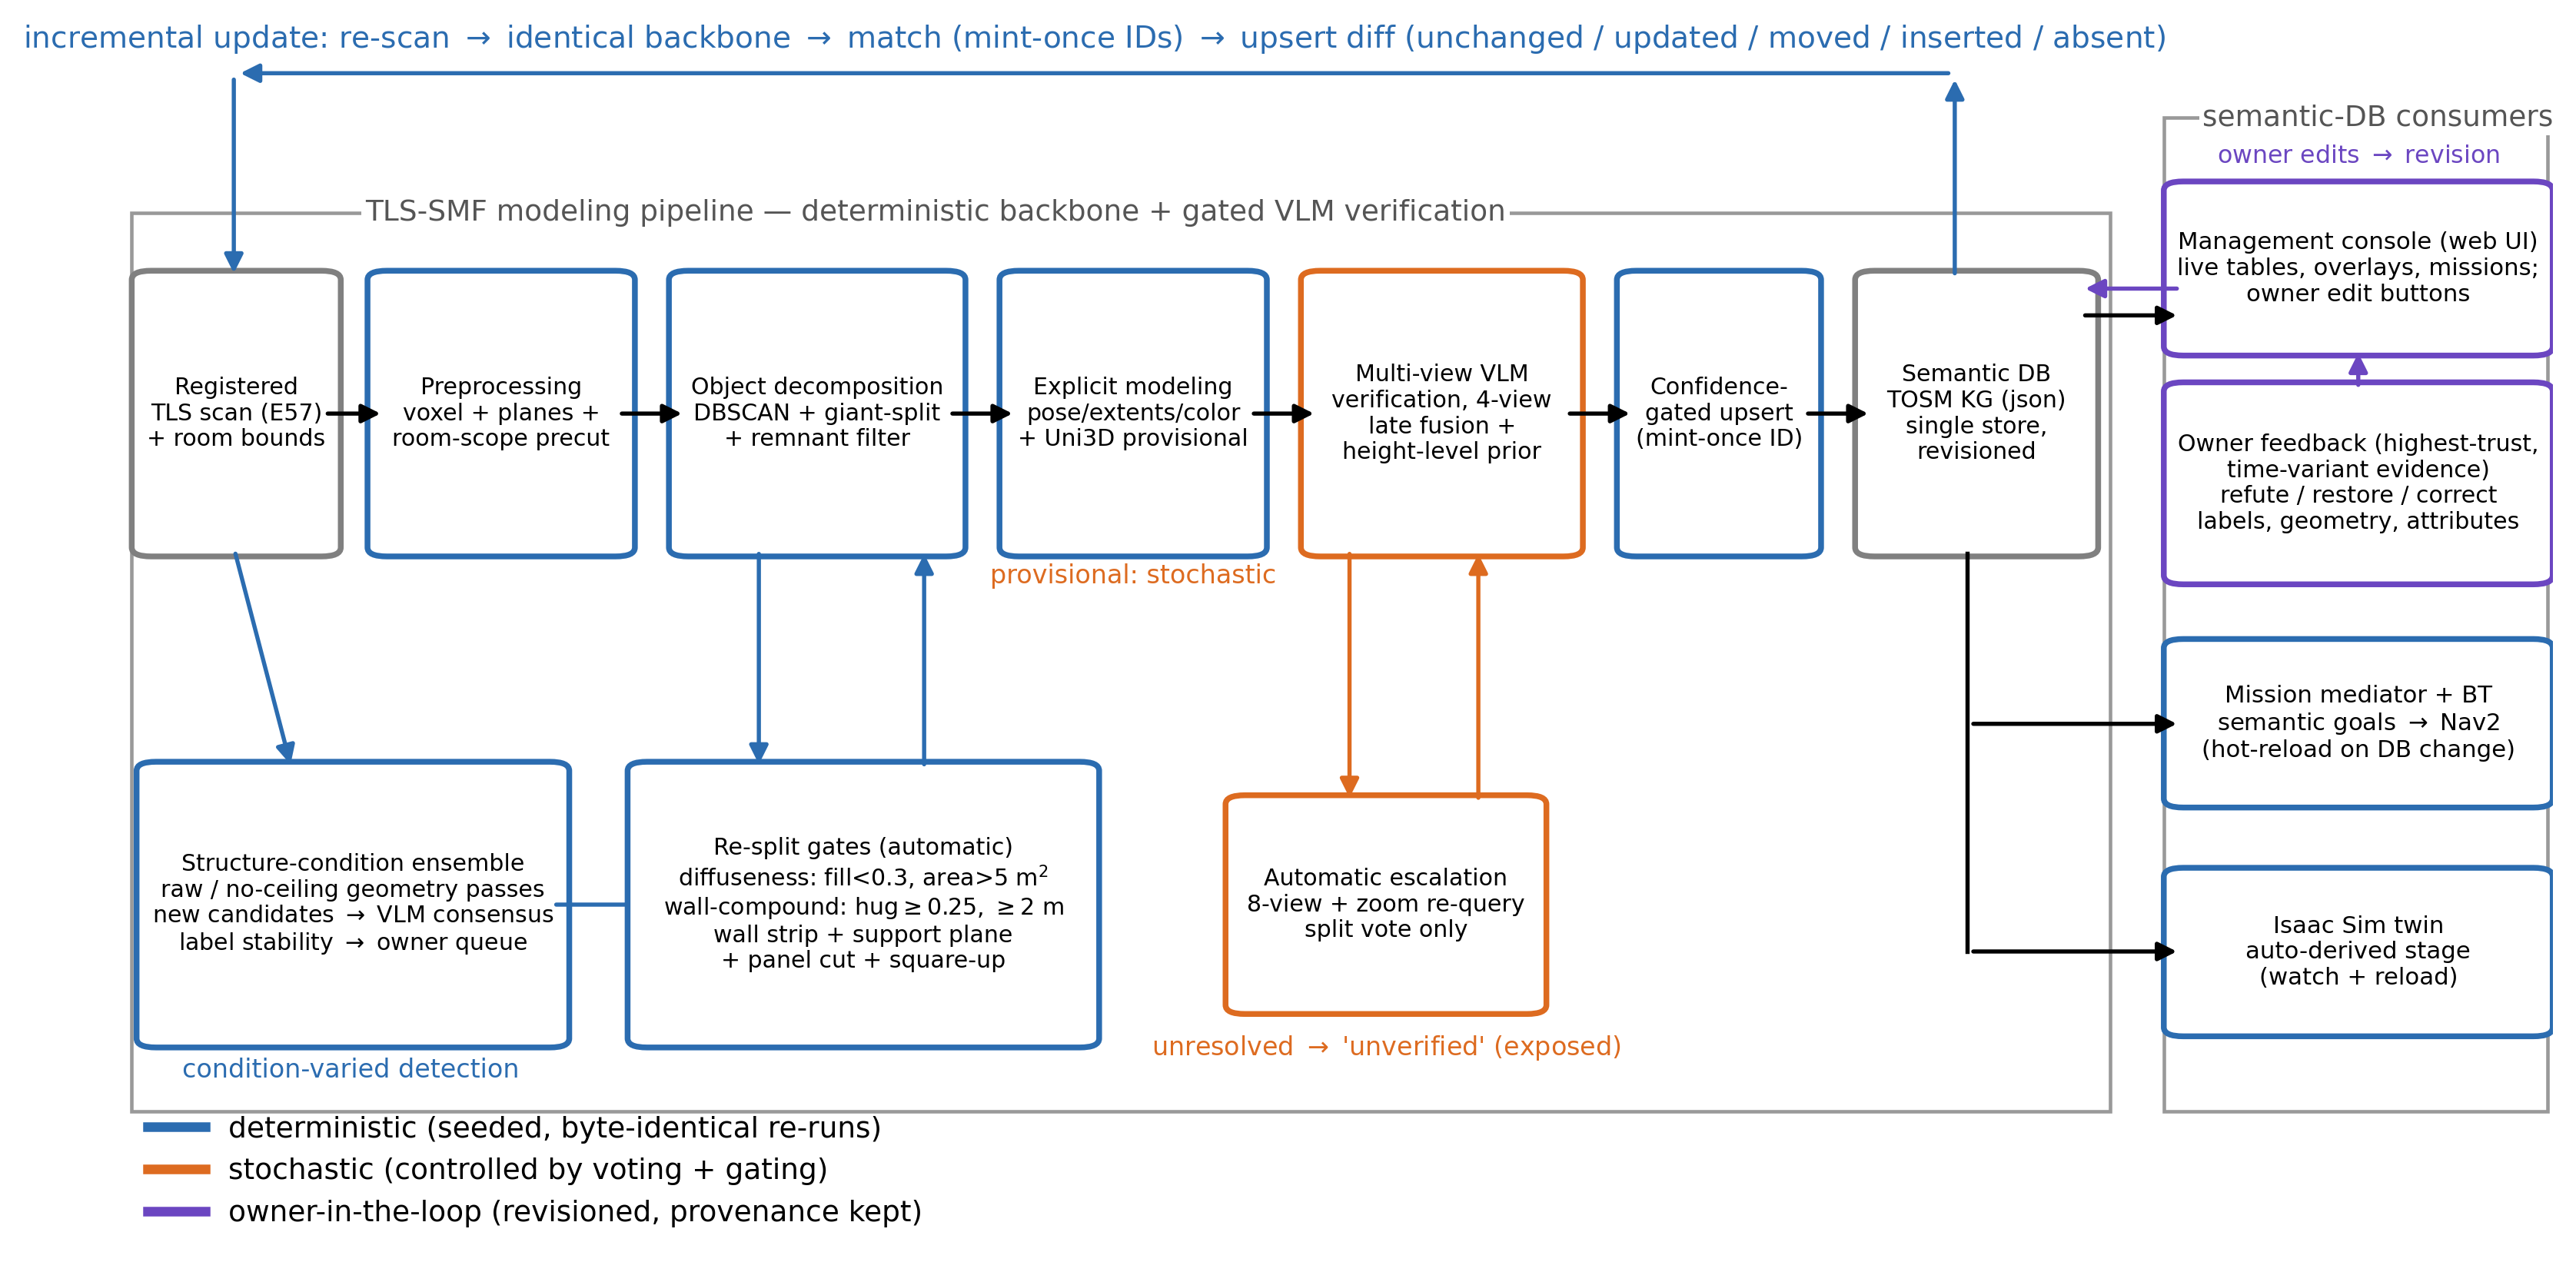
\includegraphics[width=0.95\linewidth]{figures/ele_fig1_architecture.png}
\caption{TLS-SMF architecture. Blue stages form the deterministic geometric
backbone (including the automatic re-split gates and the structure-condition
ensemble); orange stages are probabilistic semantic inference under voting,
escalation, and gating control; purple is the owner-in-the-loop revision path.
The knowledge graph is the single semantic store from which the console, the
mission mediator, and the simulation twin are derived. Four loops: escalation
(within verification), re-splitting (within decomposition), incremental update
(across scans), and owner feedback (across revisions).}
\label{fig:architecture}
\end{figure}

The color separation in the architecture is a claim boundary, not a drawing
convention. Everything in the backbone is seeded and parameter-fixed;
re-running it on the same host reproduces every retained cluster
byte-identically (Section~\ref{sec:exp-seg}). Everything downstream of the
first VLM call is stochastic; there the framework claims
\emph{control}---schema-forced outputs, multi-view voting, automatic
escalation, and confidence gating---rather than reproducibility. Each object
node carries the three TOSM description layers: a \emph{symbolic} model (type,
name, status), an \emph{explicit} model (pose, extents, yaw, color), and an
\emph{implicit} model (movability, openability, key-object status). Verified
and unverified content flows through the same graph but is separated at every
interface: verification status is part of the node schema, gating is applied
structurally at query time, and the place layer is derived from verified
objects only. The framework is fully automated \emph{after registered TLS
input}: scanner operation and vendor multi-setup registration are manual;
everything from E57 to queryable graph---including escalation decisions and
update classification---runs without human intervention, and objects the
verifier cannot resolve remain explicitly \texttt{unverified} rather than
being resolved by hand. The base algorithms are deliberately standard and
claimed as integration: RANSAC, DBSCAN, PCA modeling, open-vocabulary 3D
classification, per-view VLM querying, and the TOSM schema follow prior work.
The new mechanisms are the control structures wrapped around them.

\section{Deterministic Geometric Backbone}
\label{sec:backbone}

The backbone comprises three stages---preprocessing, decomposition with
remnant filtering, and explicit modeling with provisional
classification---connected in series so that each stage produces the
representation required by the next (Figure~\ref{fig:pipeline}). Because the
survey-grade scanner already provides a colored 3D point cloud directly, the
entire backbone operates on the point cloud without synthesizing multi-view
imagery for segmentation, preserving metric accuracy end to end. Every random
draw is seeded, so a re-run on the same host reproduces every retained cluster
byte-identically; this property is what makes verification results carryable
and diffs meaningful and, under reproducible acquisition, lets verification
cost track detected content change.

\begin{figure}[!htb]
\centering
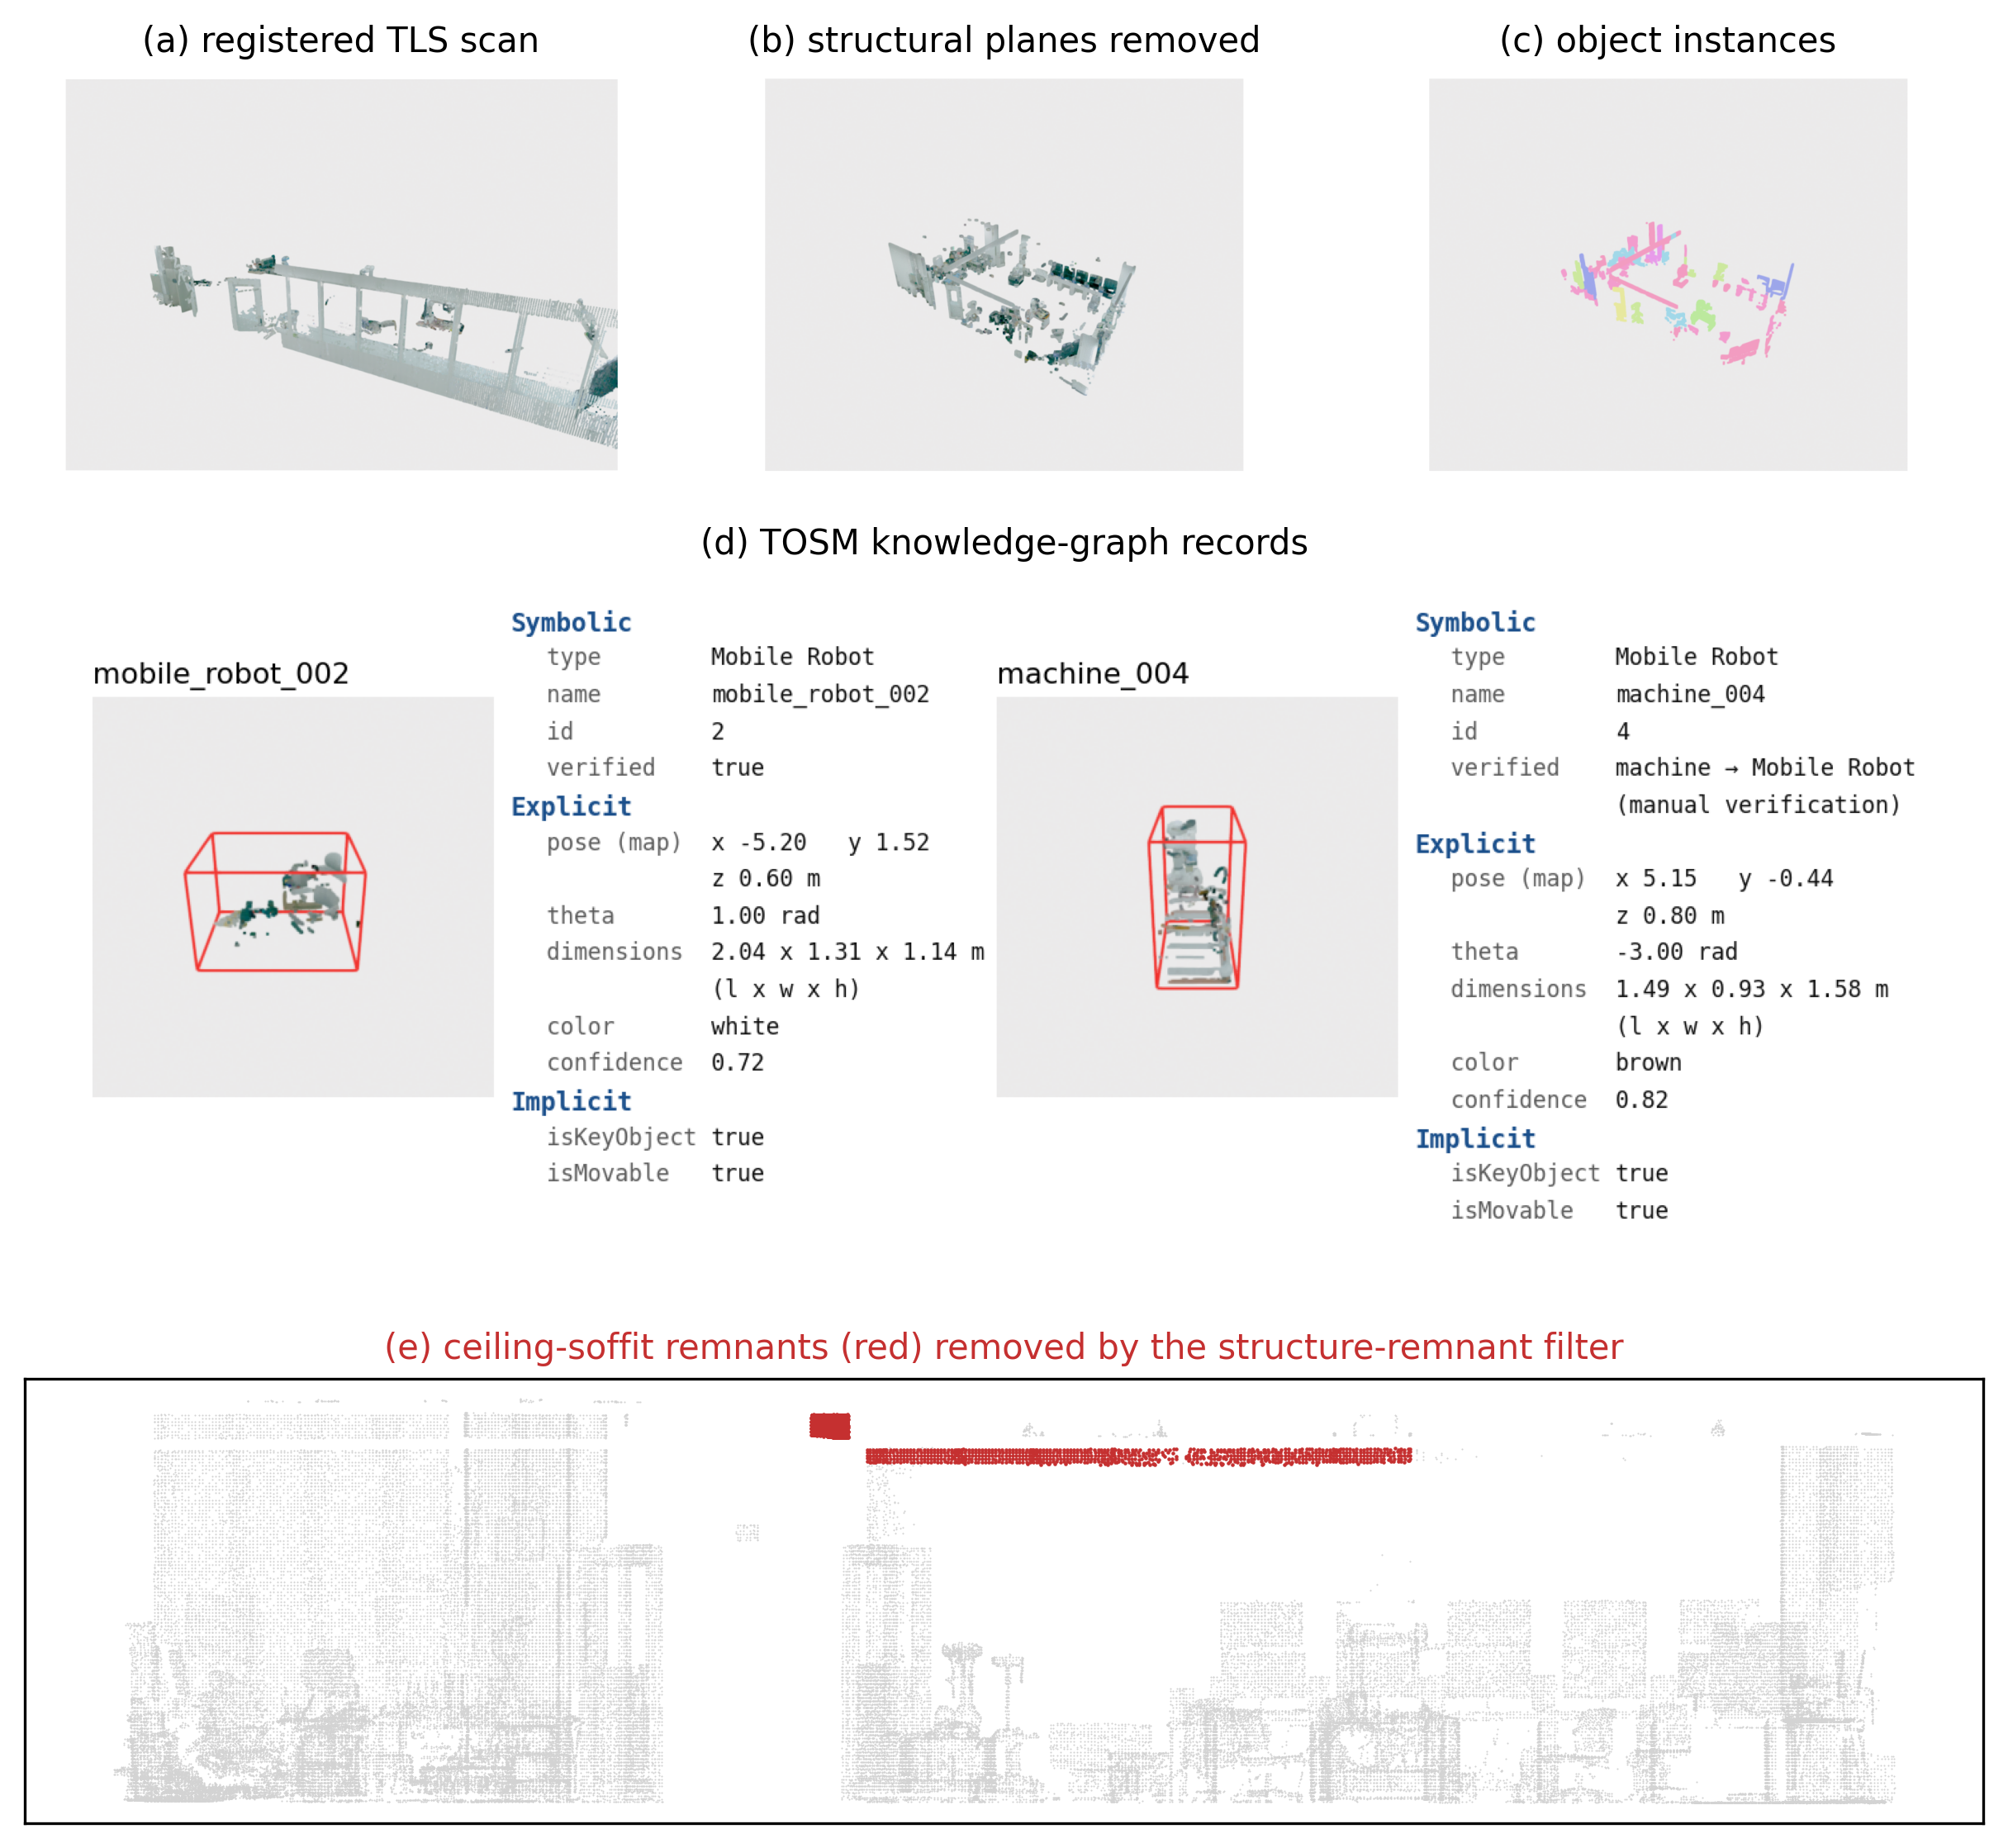
\includegraphics[width=0.92\linewidth]{figures/ele_fig2_pipeline.png}
\caption{Geometric backbone of TLS-SMF, illustrated on the test-room scene.
(a)~Registered multi-station TLS scan after preprocessing. (b)~The same cloud
after seeded-RANSAC removal of structural planes (floor, walls, ceiling).
(c)~Deterministic decomposition of the residual cloud into object instances;
identical inputs reproduce identical clusters with stable ordering. (d)~Two of
the resulting TOSM knowledge-graph records with their symbolic, explicit, and
implicit attributes. (e)~Structure-remnant filter, shown as a front elevation
of the showroom scene: the vertical soffit bands at the three-level ceiling
transitions (red) survive horizontal-plane removal and would otherwise surface
as phantom objects; the filter removes them while leaving every retained
cluster byte-identical.}
\label{fig:pipeline}
\end{figure}

\subsection{TLS Preprocessing and Structural-Plane Removal}
\label{subsec:preprocess}

The input is a registered E57 point cloud from the survey-grade scanner. When
the export contains multiple setups, the loader applies each setup's registered
pose and merges them into a single cloud; a 70M-point six-setup scan and a
pre-merged single-scan export are treated identically. The cloud is
voxel-downsampled at 3~cm---dense enough to retain object detail while bounding
the cost of all later stages---and kept in the scanner's registered frame; no
global normalization is applied. The floor height is estimated where a stage
needs it, by a robust statistic suited to that stage's input.

Structural surfaces---floor, walls, and ceiling---are then removed by
iterative RANSAC plane extraction~\cite{fischler1981ransac}. Each round draws
300 seeded random point triples, keeps the candidate with the most inliers at a
5~cm distance threshold, and refits it once by a least-squares (SVD) fit to
those inliers. A plane is removed only if it is structural by orientation:
near-horizontal ($|n_z|\ge0.85$; floors, ceilings, split ceiling levels) or
near-vertical ($|n_z|\le0.2$; walls). Interior slanted planes, which may belong
to furniture or fixtures, are preserved. The loop stops at the first of four
conditions: ten planes have been removed, fewer than 2{,}000 points remain, the
best remaining plane supports less than 4\% of the points still present, or the
best remaining plane is slanted ($0.2<|n_z|<0.85$), so that removing it would
begin carving objects. The fixed seed makes the extraction deterministic; the
pre-removal cloud is retained as a \emph{ceiling reference} for the remnant
filter below and for incremental re-runs.

\subsection{Geometric Object Decomposition and Structure-Remnant Filtering}
\label{subsec:decomposition}

The structure-free cloud is partitioned into object candidates by
fixed-parameter DBSCAN~\cite{ester1996dbscan} ($\varepsilon=0.30$~m, 100-point
minimum), followed by a \emph{conservative giant-split}: any cluster whose
horizontal footprint exceeds 2.5~m is re-clustered at a tighter
$\varepsilon=0.20$~m, and the split is accepted only if it yields at least two
sub-clusters of 100+ points---separating merged neighbors without shattering
genuinely large equipment. This stage is positioned deliberately: it is not a
novel segmentation algorithm but a \emph{reproducible decomposition designed
for verification and incremental diffing}. The requirement that motivates a
geometric, class-agnostic decomposition is that industrial and indoor
environments frequently contain fixtures, racks, and special equipment outside
the distribution of common training datasets, so segmentation bound to a
closed category set tends to miss unregistered objects or merge them
incorrectly; Section~\ref{subsec:exp-backbone} grounds this choice empirically
against learned alternatives.

\paragraph{Structure-remnant filter.}
Real buildings violate the implicit assumption that structure is planar and
objects are not. The showroom scene of Chapter~\ref{ch:experiments} has a
three-level ceiling ($z=2.48/2.18/1.95$~m): RANSAC removes each horizontal
ceiling plane, but the \emph{vertical soffit bands} at the level transitions
survive removal and surface as phantom objects
(Figure~\ref{fig:pipeline}e)---thin, wall-colored slabs that a downstream
verifier confidently misreads. The filter therefore removes any cluster that
passes all of the following tests, with thresholds fixed once and used
unchanged on every scene: (i)~soffit-scale geometry, i.e., a vertical extent
of at most 0.6~m with the bottom at least 1.5~m above the floor; (ii)~a thin
vertical planar band, i.e., a best-fit plane
with $|n_z|\le0.25$ and an RMS off-plane thickness of at most 3~cm;
(iii)~ceiling above, i.e., the footprint padded by 0.3~m contains at least 40
pre-removal points in the band from 2~cm to 45~cm above the cluster top;
(iv)~a dense horizontal layer, i.e., at least 60\% of those points concentrate
in a single $\sim$7~cm slab; and (v)~a topmost layer, i.e., the region above
that slab holds at most 20\% as many points as the slab itself, so that window
sills and wall remnants fail because the wall continues above them. Horizontal
and sloped ceiling patches are out of the filter's scope; the hybrid grid-map
structure filter of Section~\ref{sec:corrective} addresses the remaining wall,
ceiling, and outside-boundary remnants.

\subsection{Explicit Modeling and Provisional Classification}
\label{subsec:explicit}

Each cluster is summarized by an explicit model: axis extents and centroid,
yaw from the principal component of the horizontal point distribution, dominant
color, and point count. The position in the global frame is taken as the
bounding-box center and the size as the yaw-aligned extents (length, width,
height). These attributes are deterministic functions of the cluster; the
backbone's determinism claim covers geometry and these explicit attributes
only. A provisional semantic label is then attached by open-vocabulary
classification over a 30-class industrial vocabulary: the object points are
normalized and centered on a unit sphere, encoded by a point-cloud-direct
vision--language representation (Uni3D~\cite{zhou2024uni3d}), and labeled by
cosine similarity against text embeddings of the candidate categories. The
provisional label is explicitly \emph{not trusted}: the vocabulary ablation of
Section~\ref{sec:exp-ablation} shows that narrowing the vocabulary to the
deployment domain \emph{reduces} accuracy, indicating an embedding-level domain
gap rather than a class-list problem. The provisional label serves only as VLM
context and as a fallback name; every label a robot may act on must pass the
verification stage below. For each object the backbone also exports four
azimuth renders ($0/90/180/270^{\circ}$, elevation $25^{\circ}$, $512\times512$
pixels, with the 3D bounding box drawn in red), which are the input to
verification.

\section{Multi-View VLM Verification with Automatic Escalation}
\label{sec:verification}

\subsection{Schema-Forced Per-View Classification}
\label{subsec:prompts}

Verification submits each rendered view independently to a vision--language
model under a forced tool-use schema: the model must answer by calling a
declared JSON tool, so every response is schema-valid by construction and no
separate parsing or regular-expression post-processing is needed. Two prompts
are used (Figure~\ref{fig:prompt}). \emph{Prompt~1 (symbolic)}, once per
view, shows the model one render, the measured dimensions, the provisional
class, and an optional operator-supplied scene-level candidate vocabulary. The
decision rule is three-way: keep a correct label; if wrong, prefer a fitting
candidate; else emit an open-vocabulary common-noun label. Guardrails address
the failure modes of sparse point renders: measured dimensions are a hard
constraint, an oversize cluster is treated as merged objects (label the
dominant structure or \texttt{clutter}), no parts may be claimed that are not
outlined by points, thin flat objects are disambiguated among keyboard,
display, and shelf and never labeled as a ladder, and a chair requires a
visible seat pan of 0.3--0.6~m plus a backrest. The model returns a type, a
confidence, and a stated reason. \emph{Prompt~2 (implicit)}, once per object,
receives the fused type and the views and reports the TOSM implicit model:
\texttt{isKeyObject} (a fixed, distinctive landmark useful for localization),
\texttt{isMovable} (physically displaceable during normal operation), and, for
doors only, \texttt{isOpen} and \texttt{canBeOpen}. The geometric information
is provided only as context and is never modified by the model. Prompts,
decoding parameters, and the model version are recorded with every result; the
verifier model itself is a swappable component, and
Section~\ref{sec:exp-ablation} repeats the identical protocol across five
commercial VLMs.

\begin{figure}[!htb]
\centering
\fbox{\begin{minipage}{0.94\textwidth}\small
\textbf{P1 system (condensed).} Verifier for an indoor mobile robot. Input:
ONE render of a segmented 3D object (sparse laser points, red 3D box), its
classifier label \texttt{uni3d\_type}, optional candidates.
\emph{Decision rule:} (1)~KEEP a correct \texttt{uni3d\_type}; (2)~else
replace---prefer a fitting candidate, otherwise the most accurate common-noun
label; never `unknown'. \emph{Size sanity:} measured dimensions are a HARD
constraint; an oversize cluster is merged objects---label the dominant
structure or `clutter'. \emph{Sparse-render caution:} never claim parts not
outlined by points. \emph{Panel rule:} thin flat objects are keyboard /
display / shelf---never ladder. \emph{Chair gate:} visible seat pan
0.3--0.6~m plus backrest. If uncertain, keep a size-compatible label. Answer
ONLY via \texttt{report\_symbolic}.\\[2pt]
\textbf{P2 system (condensed).} From views and confirmed type, report
\texttt{isKeyObject} (fixed, distinctive landmark), \texttt{isMovable},
\texttt{isOpen}/\texttt{canBeOpen} (doors only, else null) ONLY via
\texttt{report\_implicit}.
\end{minipage}}
\caption{Condensed verification prompt design. Forced tool-use makes every
response schema-valid JSON; measured geometry is read-only context.}
\label{fig:prompt}
\end{figure}

\subsection{Confidence-Weighted Late Fusion}
\label{subsec:fusion}

The obvious multi-view strategy---feeding all views into one prompt
(\emph{early fusion})---\emph{degrades} accuracy on sparse point renders:
extra oblique speckle views invite over-confident misreadings that contaminate
the joint judgment (Section~\ref{subsec:exp-multiview}). Per-view votes are
therefore combined by confidence-weighted \emph{late fusion}, the analogue of
MVCNN-style aggregation~\cite{su2015mvcnn}. Let view $v$ return label $\ell_v$
(lowercased; no synonym mapping is applied at fusion time) with confidence
$c_v\in[0,1]$. Each candidate label accumulates the sum of the confidences of
the views that voted for it,
\begin{equation}
  s(\ell)=\sum_{v:\,\ell_v=\ell}c_v, \qquad
  \hat{\ell}=\arg\max_{\ell}s(\ell), \qquad
  \sigma=\frac{s(\hat{\ell})}{\sum_{\ell}s(\ell)},
  \label{eq:fusion}
\end{equation}
where $\hat{\ell}$ is the fused type and $\sigma$ its \emph{vote share}. A
confidence-weighted sum, rather than a view count, lets one hesitant dissenter
matter less than a confident one; a single contaminated view is simply outvoted.
The per-view votes are stored in the record, so a downstream consumer can
distinguish a 4/4 unanimous label from a 2/4 split---a free uncertainty
signal.

\subsection{Automatic Escalation and Verification Tiers}
\label{subsec:escalation}

Three outcomes follow (Figure~\ref{fig:escalation}). If the four votes are
unanimous, the object is \texttt{verified}; unanimity is empirically a strong
signal (94--100\% precision against confirmed ground truth on the industrial
scenes, Section~\ref{sec:exp-verify}), although its failure modes are
documented there as well. If the vote splits, the object \emph{escalates
automatically}: eight additional images---four diagonal azimuths and four
zoomed close-ups---are classified, and the fusion is recomputed over all twelve
votes pooled. If the post-escalation share reaches $\sigma\ge0.6$ the object
becomes \texttt{verified\_escalated}; otherwise it remains
\texttt{unverified}. The 0.6 threshold was fixed a priori as the smallest round
value that demands a clear supermajority of the confidence mass; it gates
\emph{status only}, the fused label being recorded either way, and
Section~\ref{sec:exp-verify} re-scores the stored votes across a threshold
sweep to quantify the resulting precision--recall trade-off. Crucially,
unresolved objects are not hidden, discarded, or resolved by a human: they
stay in the graph with their failed candidate label attached, and the query
interface (Section~\ref{sec:query}) is responsible for making their status
impossible to ignore. Implicit robot-facing attributes are inferred once at
fusion time from the winning view set. Escalation bounds cost: only split
votes pay for the wider view set, and per-call cost is on the order of \$0.01,
so a scene verifies for a few dollars.

\begin{figure}[!htb]
\centering
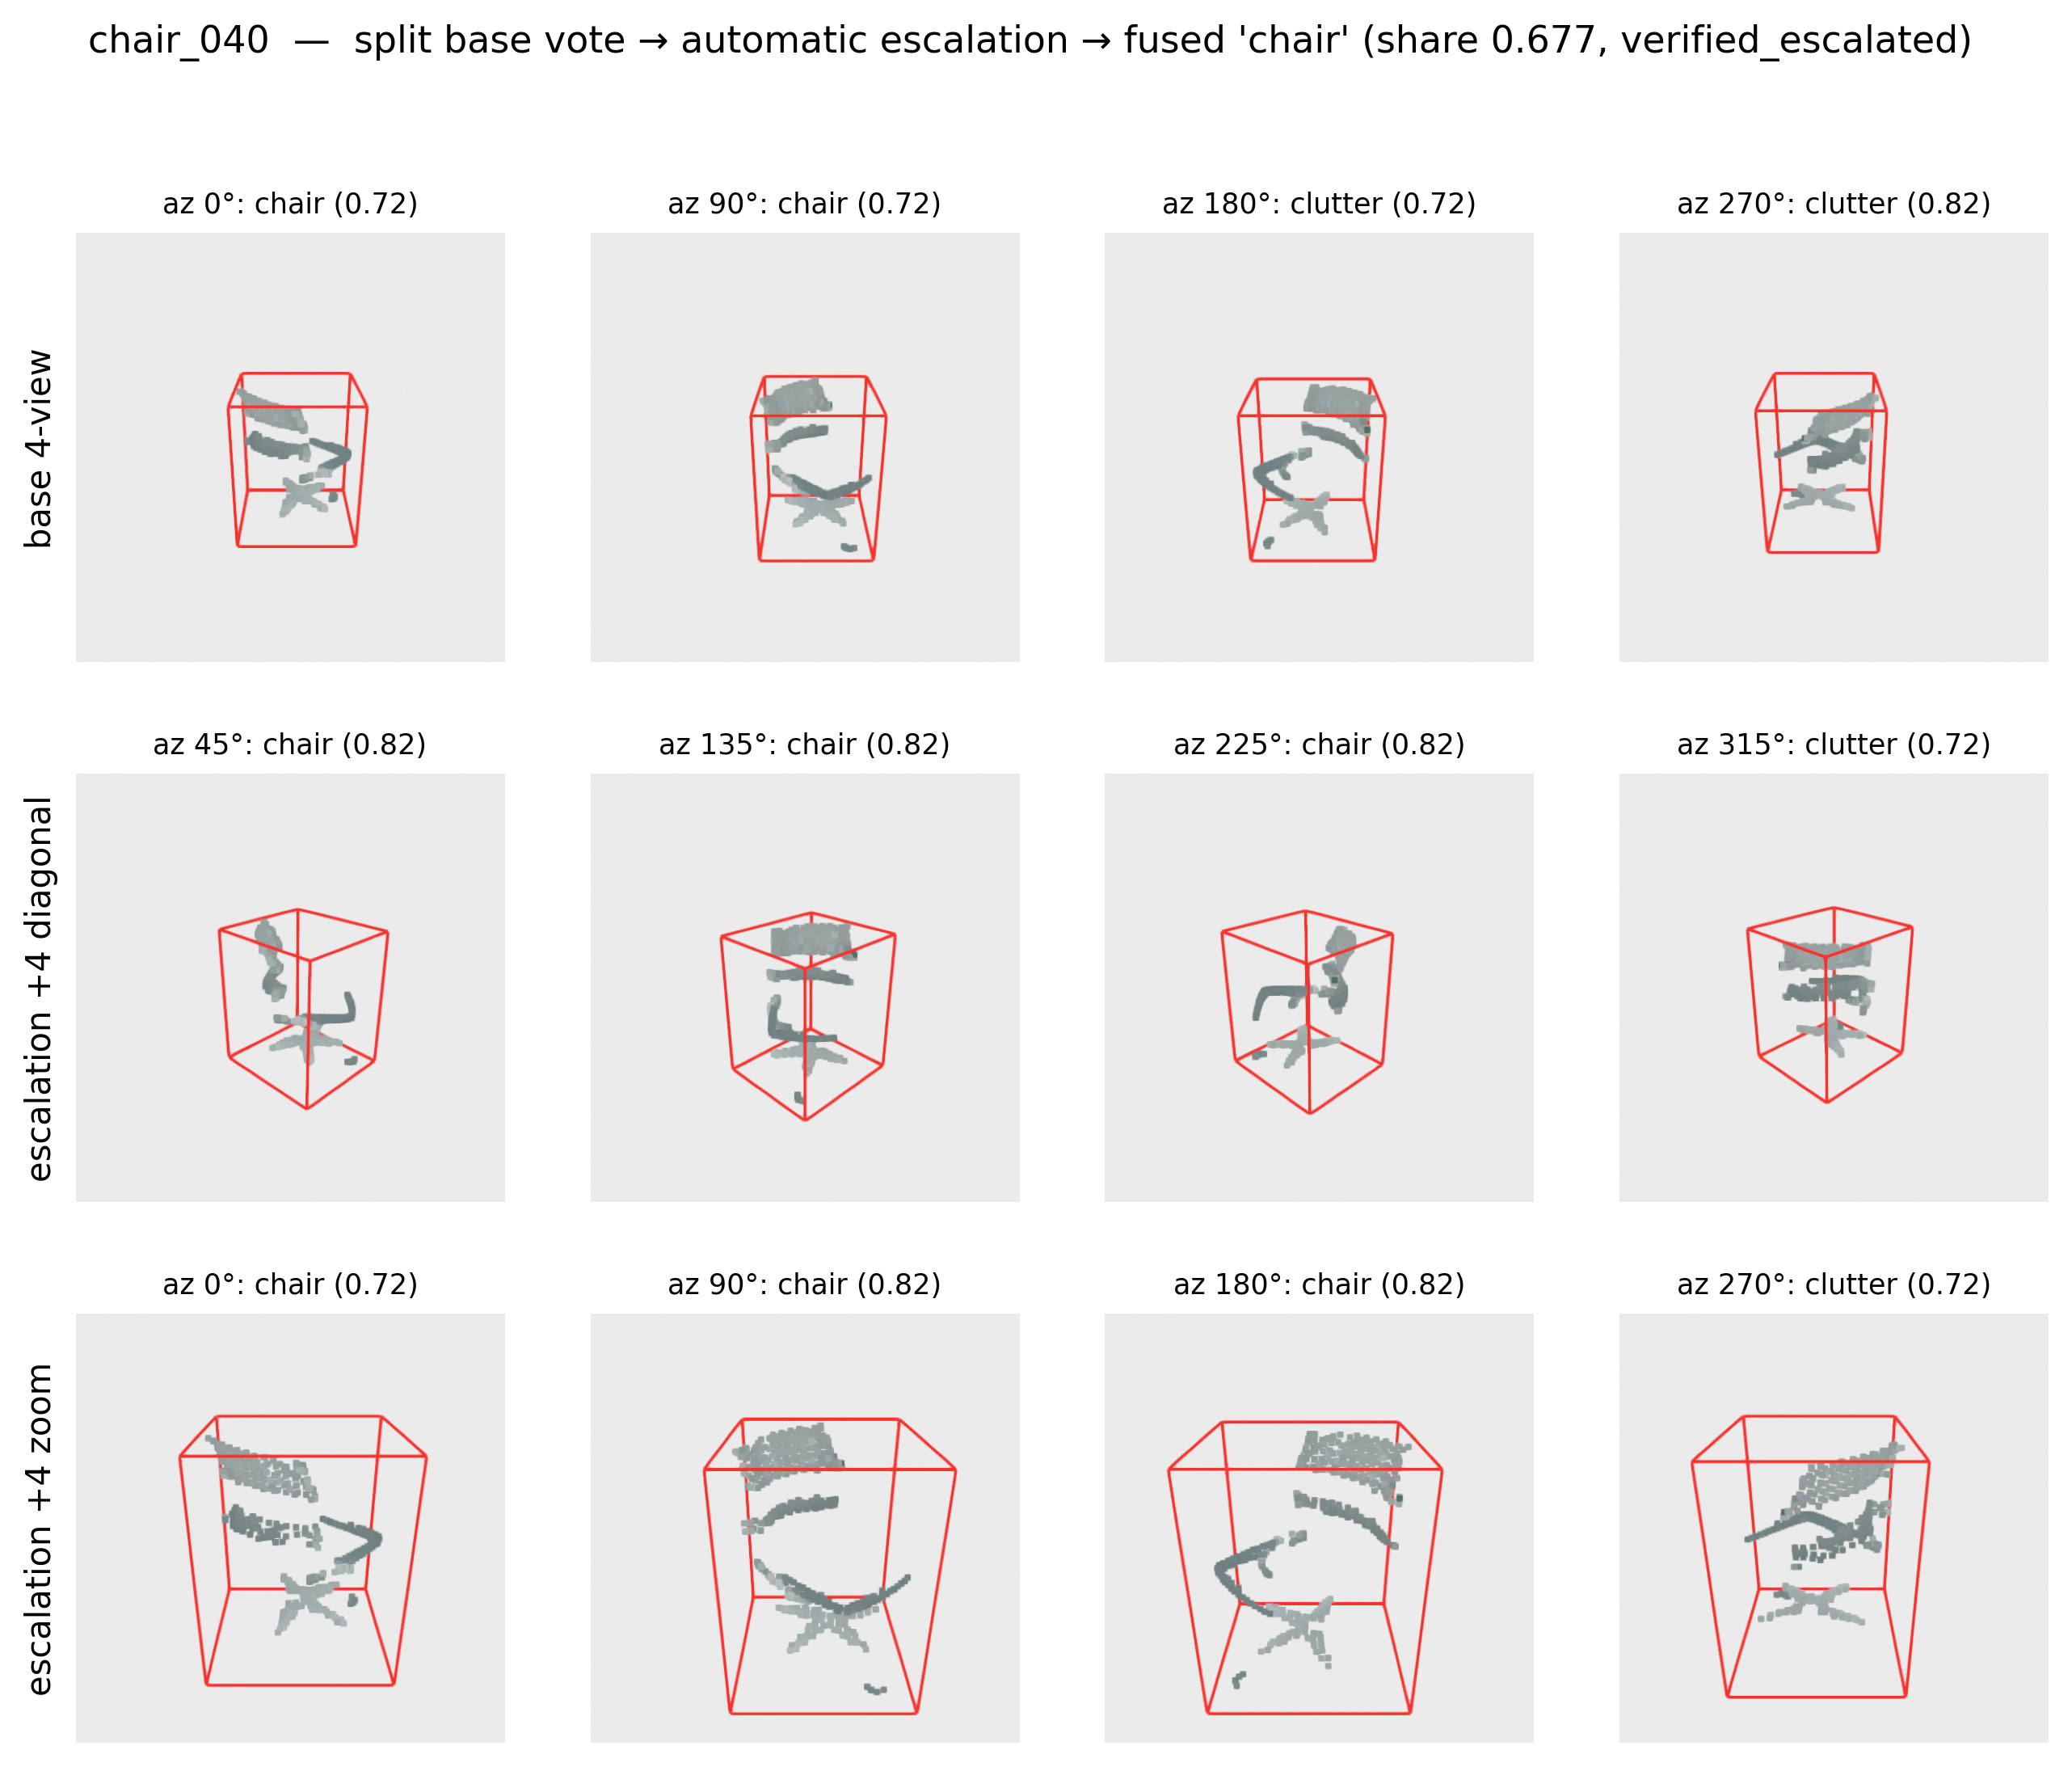
\includegraphics[width=0.95\linewidth]{figures/ele_fig3_multiview_escalation.png}
\caption{Multi-view verification and automatic escalation, with per-view
votes, fused share, and the three terminal statuses.}
\label{fig:escalation}
\end{figure}

\section{TOSM Schema and Serialization}
\label{sec:tosm-schema}

Recognized objects and places are represented in the three layers of TOSM.
Environmental elements are classified into Object and Place, subclasses of the
top-level class EnvironmentalElement, and each element carries datatype
properties corresponding to the Symbolic, Explicit, and Implicit layers as well
as object properties expressing spatial relations among elements.
Table~\ref{tab:tosm-object} defines the datatype properties of an Object and
Table~\ref{tab:tosm-place} those of a Place; Table~\ref{tab:predicates} lists
the object properties. Identifiers and categories are placed in the Symbolic
layer, scanner-measured pose, size, and color in the Explicit layer, and
information derived from inference---key-object indication, movability, door
state, place purpose---in the Implicit layer. Beyond the lineage's schema, each
node in this work carries a verification status drawn from the tier set
\begin{equation}
\begin{aligned}
\mathcal{T}=\{&\texttt{verified},\ \texttt{verified\_escalated},\ \texttt{verified\_recovery},\\
&\texttt{verified\_owner},\ \texttt{unverified},\ \texttt{refuted}\},
\end{aligned}
\label{eq:tiers}
\end{equation}
ordered by evidence source (unanimity, escalated supermajority,
agreement-gated recovery, and owner declaration at confidence 1.0), together
with provenance (per-view votes, fused share, escalation flag, model version),
a per-revision history, and \texttt{firstSeen}/\texttt{lastSeen} timestamps.

\begin{table}[htbp]
  \centering
  \caption{TOSM datatype properties for an Object. \texttt{isOpen} and
  \texttt{canBeOpen} have Door as their domain; the verification and provenance
  properties are additions of this work.}
  \label{tab:tosm-object}
  \begin{tabular}{l l l l}
    \toprule
    \textbf{Layer} & \textbf{Property} & \textbf{Domain} & \textbf{Range} \\
    \midrule
    \multirow{3}{*}{symbolicModel}
      & name & Object & string \\
      & ID   & Object & int \\
      & verificationStatus & Object & $\mathcal{T}$ (Equation~\ref{eq:tiers}) \\
    \midrule
    \multirow{5}{*}{explicitModel}
      & pose & Object & $(x, y, z, \theta)$ \\
      & coordinateFrame & Object & string \\
      & size & Object & $(l, w, h)$ \\
      & color & Object & string \\
      & heightLevel & Object & \{low, mid, high\} \\
    \midrule
    \multirow{5}{*}{implicitModel}
      & isKeyObject & Object & boolean \\
      & isMovable & Object & boolean \\
      & isOpen & Door & boolean \\
      & canBeOpen & Door & boolean \\
      & labelStability & Object & \{stable, unstable\} \\
    \bottomrule
  \end{tabular}
\end{table}

\begin{table}[htbp]
  \centering
  \caption{TOSM datatype properties for a Place, as instantiated by the
  object-grounded place layer of Section~\ref{sec:place}.}
  \label{tab:tosm-place}
  \begin{tabular}{l l l l}
    \toprule
    \textbf{Layer} & \textbf{Property} & \textbf{Domain} & \textbf{Range} \\
    \midrule
    \multirow{2}{*}{symbolicModel}
      & name & Place & string (LLM-derived from ring code) \\
      & ID   & Place & int \\
    \midrule
    \multirow{4}{*}{explicitModel}
      & boundary & Place & polygon (SLIC region) \\
      & position & Place & $(x, y, z)$ \\
      & areaTotal & Place & float \\
      & coordinateFrame & Place & string \\
    \midrule
    \multirow{3}{*}{implicitModel}
      & purpose & Place & string \\
      & keyObject & Place & Object ref \\
      & isAdjacentTo & Place & Place ref \\
    \bottomrule
  \end{tabular}
\end{table}

\begin{table}[htbp]
  \centering
  \caption{Spatial-relation object properties and the consistency rules
  enforced when they are recomputed at each upsert.}
  \label{tab:predicates}
  \begin{tabularx}{\textwidth}{l l X}
    \toprule
    \textbf{Predicate} & \textbf{Domain $\to$ Range} & \textbf{Rule enforced} \\
    \midrule
    isInsideOf & Object $\to$ Place & functional (anchor cell containment) \\
    isNextTo & Object $\to$ Object & symmetric; kept only within the same place \\
    isOn / isAboveOf & Object $\to$ Object & asymmetric; requires rotated-footprint overlap \\
    isAdjacentTo & Place $\to$ Place & symmetric \\
    isKeyObjectOf & Object $\to$ Place & functional; refuted objects excluded \\
    isMovable / isStatic & Object $\to$ bool & mutually exclusive \\
    \bottomrule
  \end{tabularx}
\end{table}

Instead of the OWL representation used by prior work, the graph is serialized
in a VDA~5050-based JSON format~\cite{vda5050} for compatibility with downstream
robot-operation standards, and exported in parallel as map-scoped Neo4j Cypher
so that multiple sites and epochs coexist in one database. VDA~5050 specifies
the communication between automated guided vehicles and a master control; this
work borrows its message schema to express each semantic object as a JSON
record composed of header metadata (manufacturer, serial number, timestamp,
version) and an object array, so that the semantic model can be consumed by an
AGV control pipeline without a separate conversion step. TOSM fields with no
standard slot travel in the extensible \texttt{properties} map, so consumers
that only know the base schema can still read the message
(Table~\ref{tab:mapping}); Code~\ref{code:record} shows an example record.

\begin{table}[htbp]
  \centering
  \caption{TOSM $\to$ VDA~5050-style JSON field mapping.}
  \label{tab:mapping}
  \begin{tabularx}{\textwidth}{l l X}
    \toprule
    \textbf{TOSM model} & \textbf{Element} & \textbf{JSON field} \\
    \midrule
    symbolic & class & \texttt{type} \\
             & name / identity & \texttt{name}, \texttt{id} \\
             & verification status & \texttt{properties.verificationStatus} \\
    explicit & position, height & \texttt{poseX}, \texttt{poseY}, \texttt{properties.poseZ} \\
             & orientation, size & \texttt{poseTheta}, \texttt{dimensions\{l,w,h\}} \\
             & color & \texttt{color} \\
    implicit & landmark / movability & \texttt{properties.isKeyObject}, \texttt{isMovable} \\
             & door state & \texttt{properties.isOpen}, \texttt{canBeOpen} \\
    --       & VLM audit trail & \texttt{properties.viewVotes}, \texttt{symbolicReason}, \texttt{confidence} \\
    \bottomrule
  \end{tabularx}
\end{table}

\begin{quote}
\small\ttfamily
\begin{verbatim}
{
  "manufacturer": "CASELAB", "serialNumber": "...", "version": "0.0.0",
  "semanticObjects": [
    {
      "type": "control panel", "id": "0", "name": "control_panel_000",
      "poseX": 6.49, "poseY": 4.11, "poseTheta": -3.12,
      "dimensions": { "length": 5.75, "width": 0.71, "height": 3.24 },
      "color": "brown", "confidence": 1.0,
      "properties": {
        "poseZ": 0.63, "coordinateFrame": "map", "source": "DBSCAN+Uni3D",
        "verificationStatus": "verified", "viewVotes": [...],
        "isKeyObject": true, "isMovable": false,
        "isOpen": null, "canBeOpen": null,
        "symbolicReason": "...",  "implicitReason": "..."
      }
    }
  ]
}
\end{verbatim}
\end{quote}
\noindent\textbf{Code 4.1.}\quad Example of a semantic-object JSON record
(VDA~5050 message format; some values abbreviated).
\label{code:record}
\medskip

\section{Object Identity Matching}
\label{sec:matching}

The update problem is an \emph{identity} problem before it is a geometry
problem: a robot that plans against node IDs needs yesterday's chair to be
today's chair. The policy is \textbf{mint-once}: a node ID is minted when an
object first enters the graph---derived from a fingerprint of its birth-time
anchor (map, position, extent)---and never changes afterwards. The fingerprint
is a candidate-retrieval key, not the identity itself; after minting, matching
alone carries identity forward. Matching between a new scan's records and
existing nodes runs in two passes.

\begin{enumerate}
\item \textbf{Spatial pass.} A record matches a node if their 3D centroids
agree within 0.5~m and each of the three extents agrees within a per-axis
tolerance of $\max(0.3\cdot\max(d_{\mathrm{old}},d_{\mathrm{new}}),\,0.15\,\mathrm{m})$---a
30\% relative band with a 15~cm absolute floor so that small objects are not
over-constrained. No type constraint applies in this pass; a changed label on a
geometrically stable object is recorded as an update, not a new object. Matches
update pose and extents in place (\texttt{unchanged}/\texttt{updated}).
\item \textbf{Move pass.} Remaining records match remaining nodes of the
\emph{same type} with dimensions consistent under the same tolerance, within a
6~m horizontal search radius, producing \texttt{moved} nodes with preserved
IDs. Generic types (\texttt{clutter}, \texttt{unknown}) are excluded from this
pass: a generic label carries too little identity for displacement claims, and
the real two-epoch data showed that admitting them fabricates 2--5~m ``moves''
between unrelated piles.
\end{enumerate}

When several nodes satisfy the predicate for one record, the record claims the
node with the smallest horizontal centroid distance; when several records
compete for one node, the first claim wins and the node is removed from the
candidate pool. Assignment is therefore greedy in the backbone's deterministic
cluster order, so the assignment itself is reproducible. The thresholds encode
physical priors rather than tuned values: 0.5~m is below the smallest
inter-object spacing a scan-to-scan pose drift is expected to produce for a
stationary object and far above the $\le$5~cm registration residual; the
30\%/0.15~m extent band absorbs partial-view truncation without admitting
differently sized objects; and 6~m bounds a within-room relocation. Records
that match nothing are minted as new nodes (\texttt{inserted}); nodes that no
record claims are marked \texttt{absent} but retained with their full history,
so an object that returns later resumes its original identity. Formally, the
match function is
\begin{equation}
m(n,r)=\mathbb{1}[\lVert p_n-p_r\rVert_{3\mathrm{D}}\le0.5]\cdot
\prod_{k\in\{l,w,h\}}\mathbb{1}\bigl[\,|d_{n,k}-d_{r,k}|\le
\max(0.3\max(d_{n,k},d_{r,k}),0.15)\bigr],
\label{eq:match}
\end{equation}
with the move-pass variant substituting a 6~m horizontal bound and an
exact-type, non-generic constraint. The upsert decision for each record--node
pair follows the deterministic cascade \emph{match} $\rightarrow$ \emph{move}
$\rightarrow$ \emph{insert}, with unclaimed nodes marked \emph{absent}; every
transition appends to the node's history, and no node is ever deleted
(Figure~\ref{fig:upsert}).

\begin{figure}[!htb]
\centering
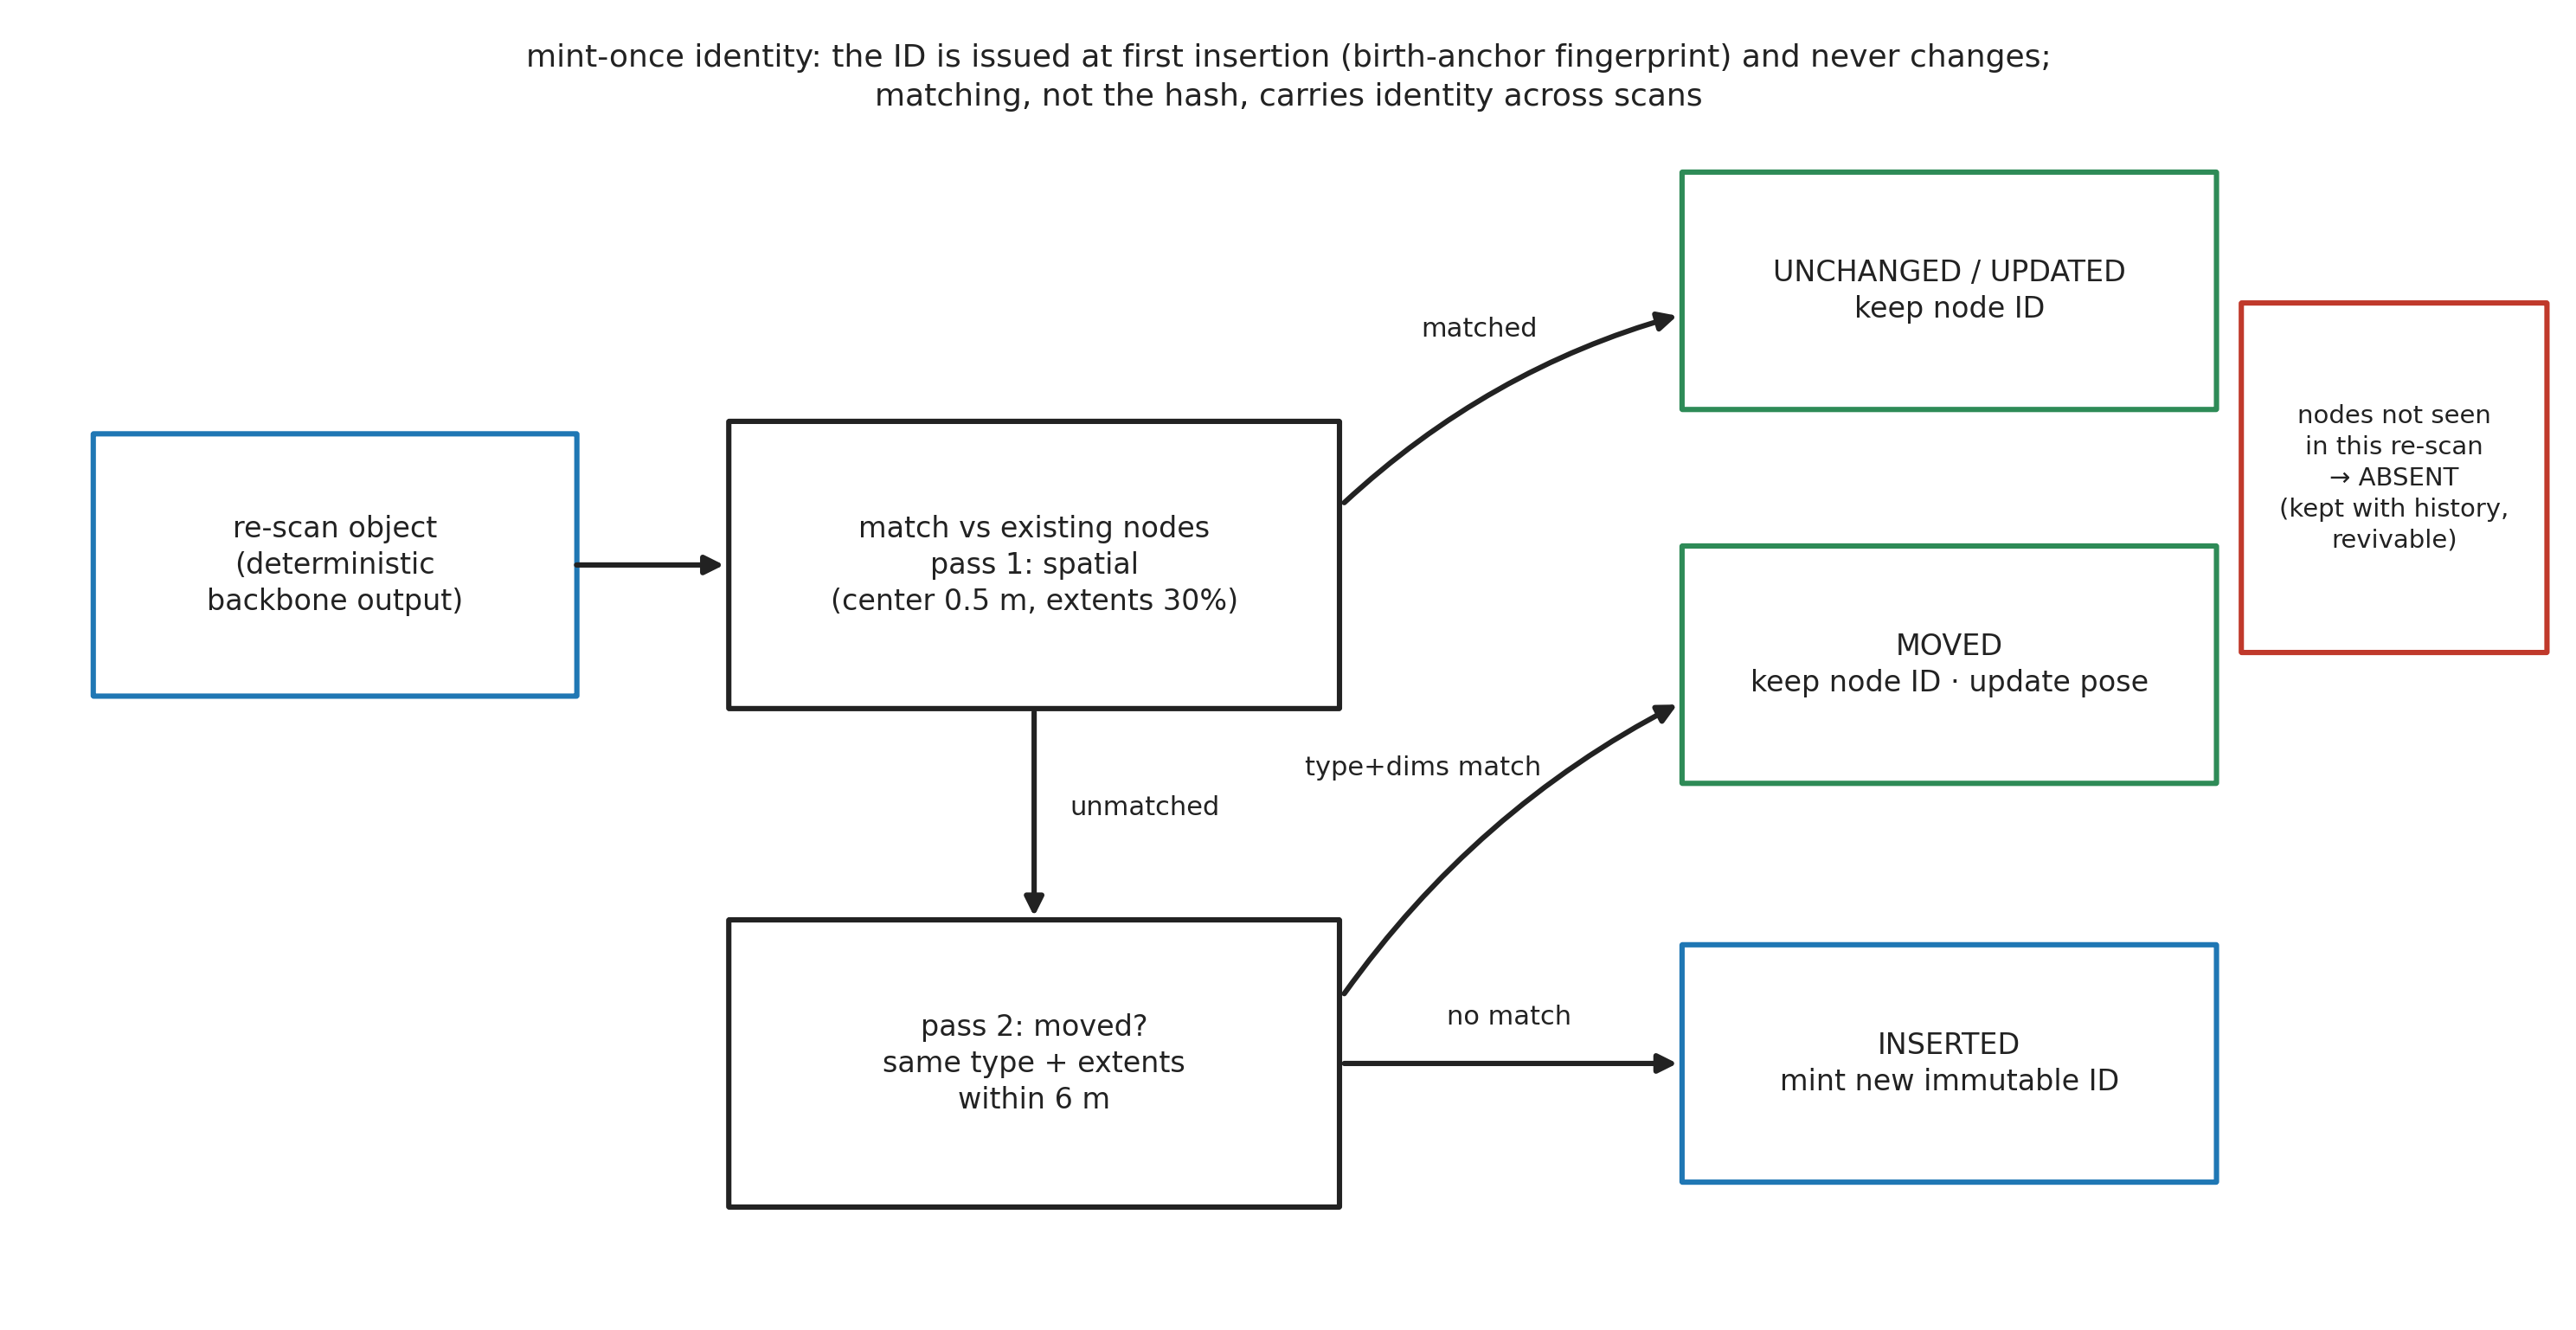
\includegraphics[width=0.9\linewidth]{figures/ele_fig5_identity_upsert.png}
\caption{Identity matching and confidence-gated upsert: mint-once IDs,
two-pass matching, and the five node outcomes across a re-scan.}
\label{fig:upsert}
\end{figure}

\section{Confidence-Gated Graph Upsert}
\label{sec:upsert}

Each scan epoch applies its matched record set to the knowledge graph as a
node-level upsert---no rebuild. Edges (spatial relations recomputed from
explicit models) are scoped to the map and revision and organized by the place
layer: \texttt{isNextTo} is kept only between objects of the same place
(proximity across a place boundary is expressed at the place level as
\texttt{isAdjacentTo}), vertical relations \texttt{isOn}/\texttt{isAboveOf}
must pass a rotated-footprint overlap test (a separating-axis check that
discards the long-range stacked relations oversized merged clusters otherwise
produce), and each place designates a key object (the VLM's implicit
\texttt{isKeyObject} among verified members, falling back to the most confident
specific-type verified member; objects refuted by owner feedback are excluded
from designation while remaining in the graph as annotated errors)
(Figure~\ref{fig:relmap}). Because unchanged objects reproduce byte-identical
clusters, their verification results are carried over by content hash and an
identical-input repeat scan costs \emph{zero} VLM calls; a changed scan of the
same acquisition quality pays only for changed clusters. The carry-over is
conditional on reproducible acquisition: when scan quality itself changes
between epochs, no cluster hashes match and the epoch pays full verification
cost (Section~\ref{sec:exp-update}). All numeric constants of
Sections~\ref{sec:backbone}--\ref{sec:upsert} were fixed on the development
epochs and applied unchanged to the later epoch and to the cross-floor scene.

\begin{figure}[!htb]
\centering
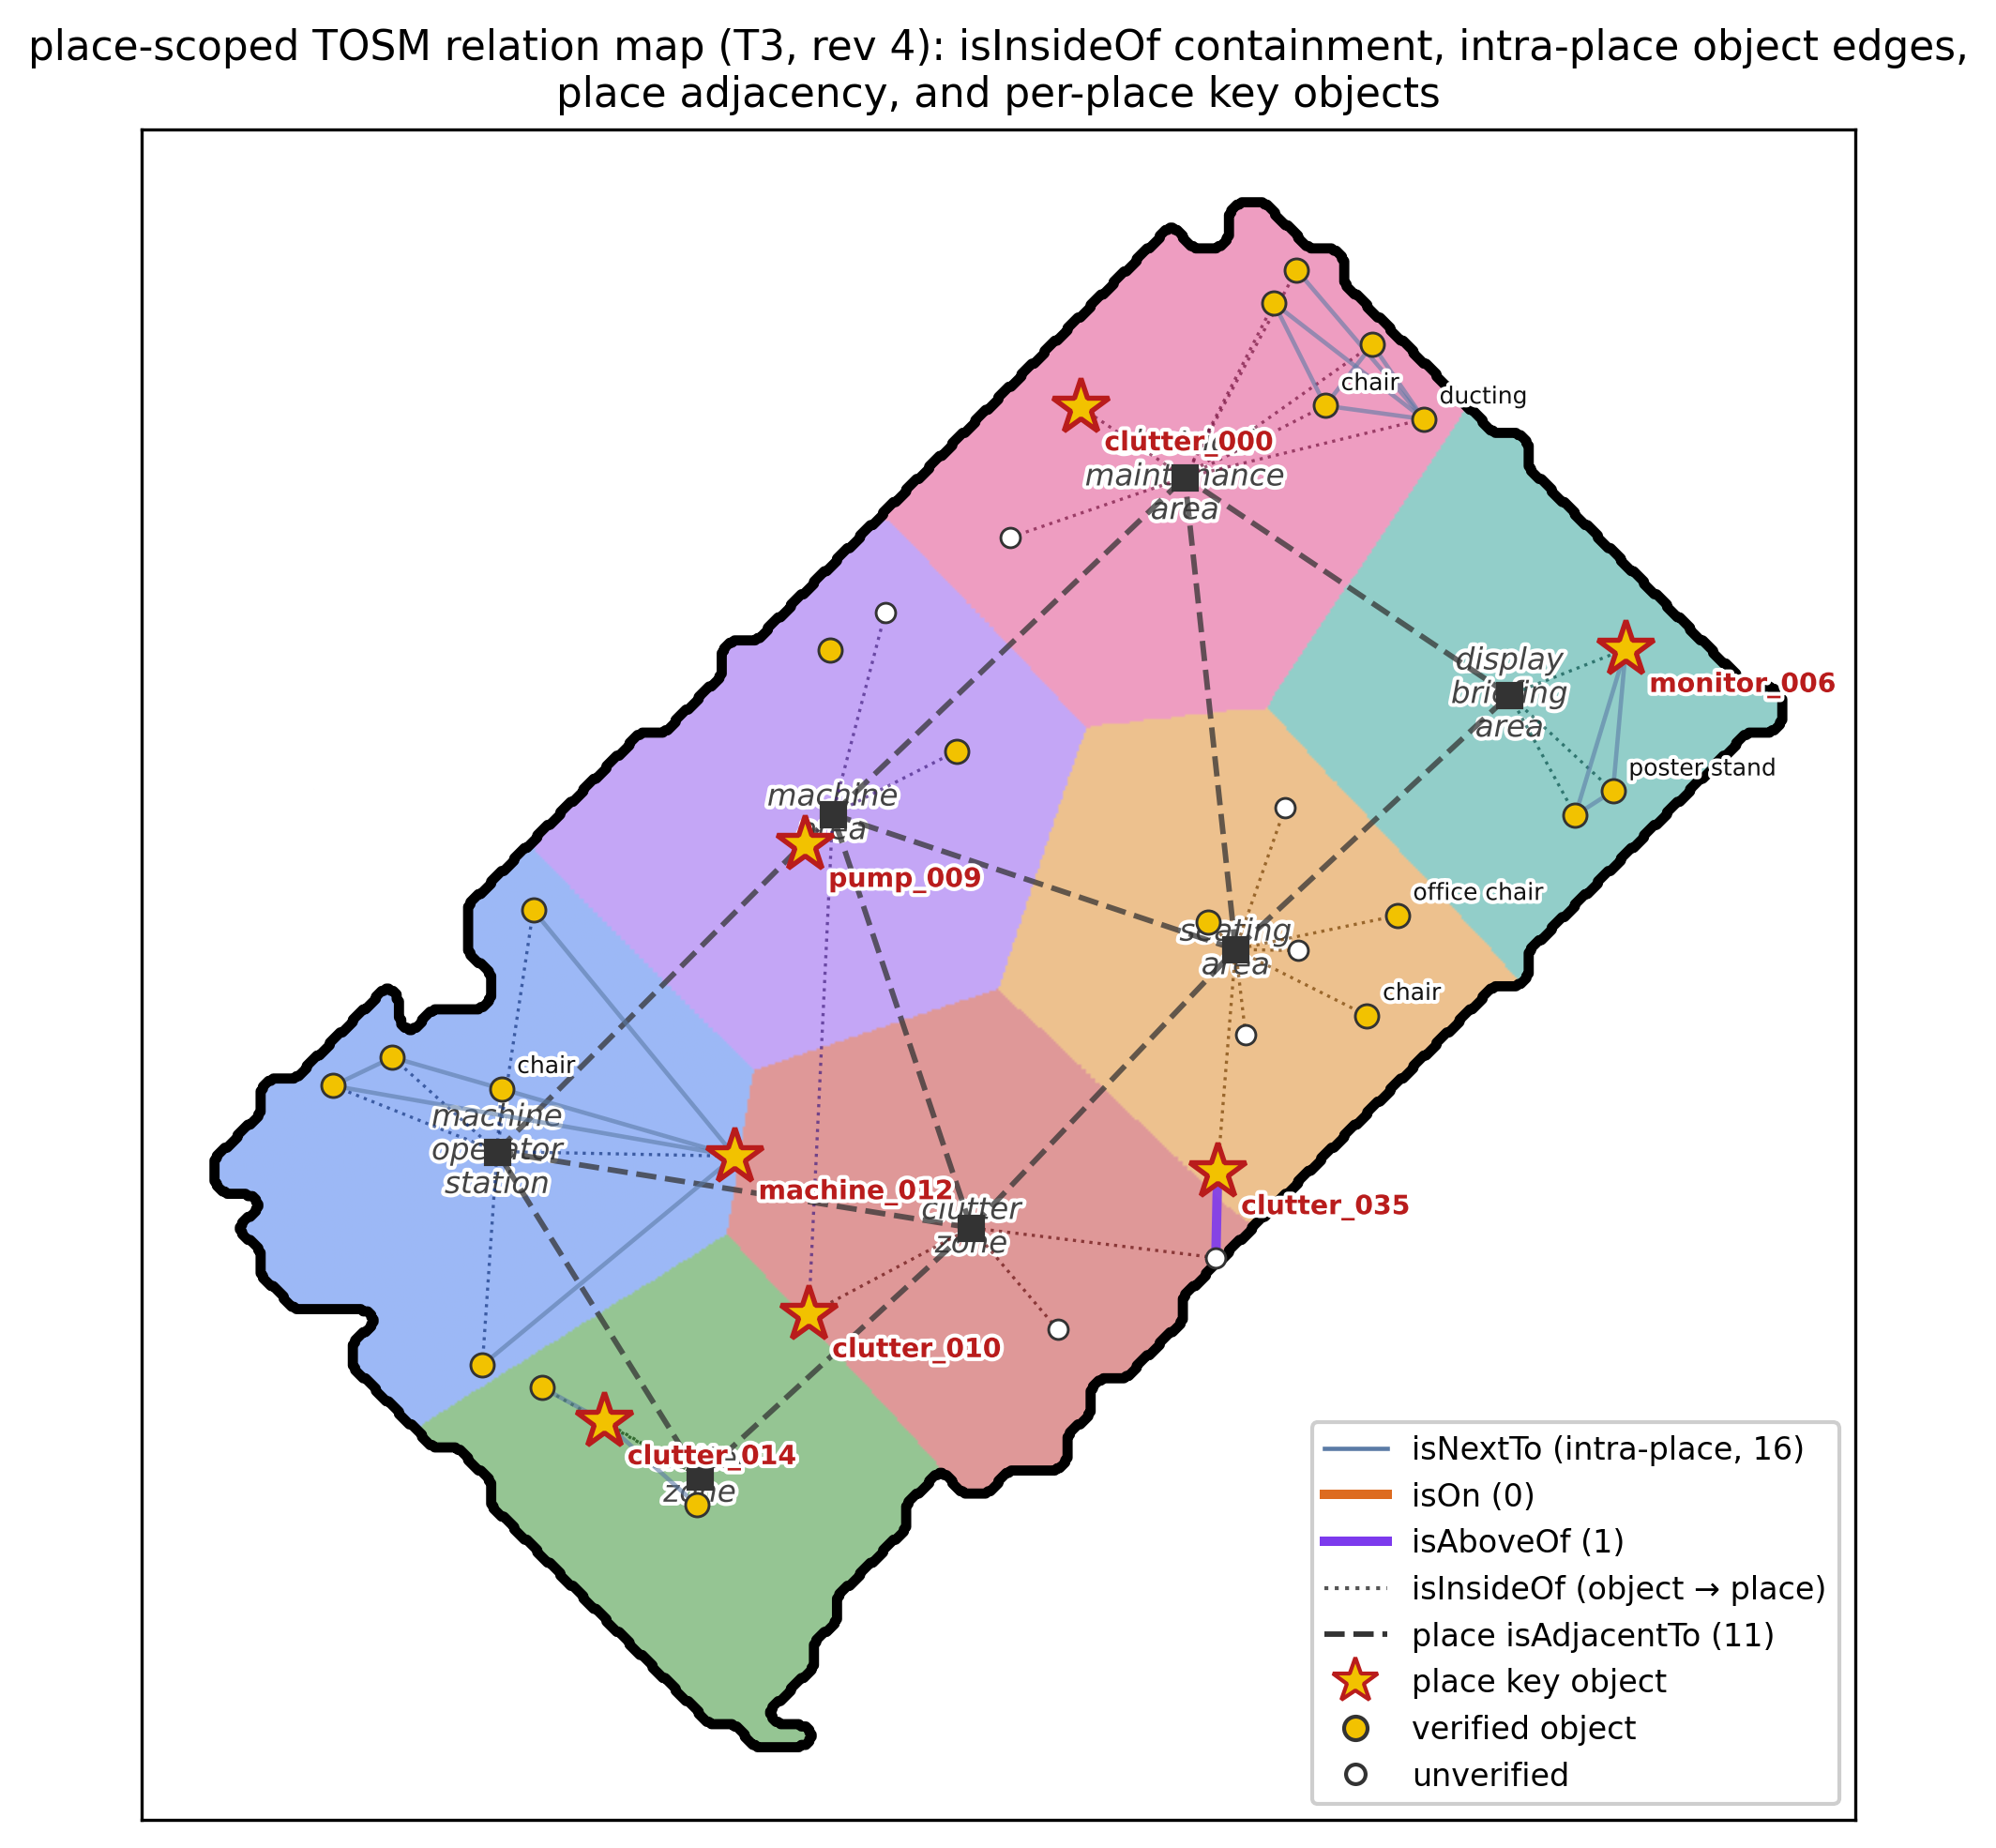
\includegraphics[width=0.85\linewidth]{figures/ele_fig12_relations_map.png}
\caption{Place-scoped TOSM relation map over the place layer of
Figure~\ref{fig:placemap}: dotted object$\rightarrow$place \texttt{isInsideOf}
containment, intra-place \texttt{isNextTo} edges, vertical
\texttt{isOn}/\texttt{isAboveOf} relations, dashed place \texttt{isAdjacentTo}
edges between region centroids, and per-place key objects (named stars).}
\label{fig:relmap}
\end{figure}

\section{Corrective Decomposition Layers and Owner Feedback}
\label{sec:corrective}

The backbone of Section~\ref{sec:backbone} is deliberately conservative, and
its characteristic failures---diffuse residual webs, wall-flush compounds
amputated by structure removal, structure noise that survives plane removal,
and real objects absorbed into \texttt{clutter}---are corrected by five layers.
The first four are automatic and run inside the frozen pipeline on every epoch;
the fifth is the human-in-the-loop channel. All were developed in response to
failures observed on the development epochs; their definitions, triggers, and
parameters were frozen before the cross-floor evaluation and require no
per-scene adjustment at execution.

\begin{enumerate}
\item \textbf{Diffuseness-gated re-split.} Trigger: a cluster whose 2D
occupancy fill (10~cm grid) is below 0.30 while its footprint exceeds
5~m$^2$---real objects fill 0.5--0.85. The cluster is re-decomposed by
occupancy-core erosion: grid cells with $\ge$8 points and $\ge$3 occupied
8-neighbors seed connected components; components with $\ge$250 points survive.
Compounds are further split at the support plane (the $z$-histogram peak
0.5--0.95~m above floor), with grounded cells spanning $>$1.3~m vertically
treated as legs or poles, and under-slab fragments re-attached at $\ge$60\%
footprint overlap. An evidence gate ($\ge$250 points, $\ge$5~m$^2$ or 12~m$^2$
for desk banks, $\ge$0.15~m height) keeps only physically plausible
sub-objects.
\item \textbf{Wall-compound gate.} Trigger: $\ge$25\% of a cluster's points
within 0.12~m of the exploration-grid wall line over a span of $\ge$2~m, with
$\ge$250 points protruding off-wall, and the cluster not diffuse. The wall
band is stripped, the support plane is detected as above, and the panel band
is cut at density valleys along the wall, yielding unit-level decomposition of
wall-mounted equipment. A final \emph{panel square-up} pass re-assigns every
compound point that falls inside a panel unit's bounding box, padded by 6~cm
horizontally and 5~cm vertically, back to that unit; it is
instance-segmentation finishing with no semantic input.
\item \textbf{Structure-condition ensemble.} Trigger: every epoch. The
geometric pass is repeated under three structure-removal conditions (none /
ceiling-only / full); clusters found under an alternative condition but absent
from the production set become new candidates, and only those are sent to
verification. Cross-condition label agreement is stored per object as a
\texttt{labelStability} attribute that prioritizes owner review;
cross-condition \emph{voting} is deliberately not used to fuse labels, because
verifier biases proved correlated across conditions.
\item \textbf{Hybrid grid-map structure filter.} Trigger: every epoch, after
clustering. Each cluster is registered against the exploration occupancy grid
of Chapter~\ref{ch:mapping}---an independent, drift-free wall prior---and
flagged by the first matching rule of a fixed cascade: outside-room ($>$50\% of
points beyond the filled room polygon), ceiling fixture (bottom $>$2.0~m above
floor), wall remnant (fraction of points within 0.15~m of the nearest grid wall
line $>$0.6 with PCA minor extent $<$0.22~m and a horizontal minor axis), or
full-height wall band ($z$-span $>$2.5~m, per-meter-segment median thickness
$<$0.3~m, along-wall length $>$2~m---the length condition spares wall-mounted
panels). Flagged clusters are removed upstream of verification.
\item \textbf{Owner feedback and gated recovery.} The management console
exposes four operations, each applied as a normal graph revision with
history: \emph{declare} (sets \texttt{verified\_owner} at confidence 1.0),
\emph{refute} (sets \texttt{refuted}, presence \texttt{absent}, and exclusion
from key-object designation), \emph{correct} (label or attribute in place, the
VLM verdict retained in provenance), and \emph{re-verify}. Recovery
re-verification re-asks the verifier with \texttt{clutter} treated as
\emph{unidentified}, in two independent passes (open vocabulary; site
vocabulary plus provisional candidates); a recovered label is adopted---as
\texttt{verified\_recovery}---only when the two passes agree under canonical
synonym matching, or a pass agrees with the cluster's own base label, and the
label is not \texttt{clutter}; a focused tie-break pass re-asks with exactly
the two disputed labels and is accepted only at confidence $\ge$0.6. A coarse
three-level height attribute (low/mid/high relative to the 2D-lidar scan plane
and the ceiling) is injected as a hard physical constraint in these passes and
stored as a queryable explicit attribute.
\end{enumerate}

The owner is not a fallback annotator but the highest-trust evidence source in
a permanently open loop: owner ground truth is itself \emph{time-variant}
(an object refuted as absent may later be declared present again when the room
changes), which is why feedback is recorded as evidence with history rather
than as immutable truth, and why one correction propagates through the object,
relation, place, scene, and mission layers at once from a single write.

\section{Query Interface with Structural Gating}
\label{sec:query}

The graph is queried through an LLM that receives a
serialized view of the relevant nodes. The naive design---instructing the
model not to assert unverified labels---fails in practice: in the benchmark of
Section~\ref{sec:exp-ablation} the instructed model still asserted trap labels
in 3 of 4 cases. The framework therefore \emph{gates by construction, not
exhortation}: in the query-time view, every unverified node's type is demoted
to \texttt{unknown}, and the failed candidate label is moved to a separate
\texttt{failedCandidateType} field whose semantics (``a classifier guess that
did not survive verification'') are stated in the schema, not in behavioral
instructions (Figure~\ref{fig:cards}). With the gate in the data rather than
the prompt, the model cannot assert an unverified label without visibly
contradicting its input. Traps whose label was wrongly \emph{verified} lie
beyond any status-based gate---a bound quantified in
Section~\ref{sec:exp-query}. In interaction, the gate makes confidence part of
the answer rather than metadata: asked whether there is a keyboard in the room,
the system asserts a verified keyboard with its location, while an unverified
one yields ``an object at $(x,y)$ was proposed as a keyboard by the classifier
but did not pass verification''---an answer a robot can act on conservatively.

\begin{figure}[!htb]
\centering
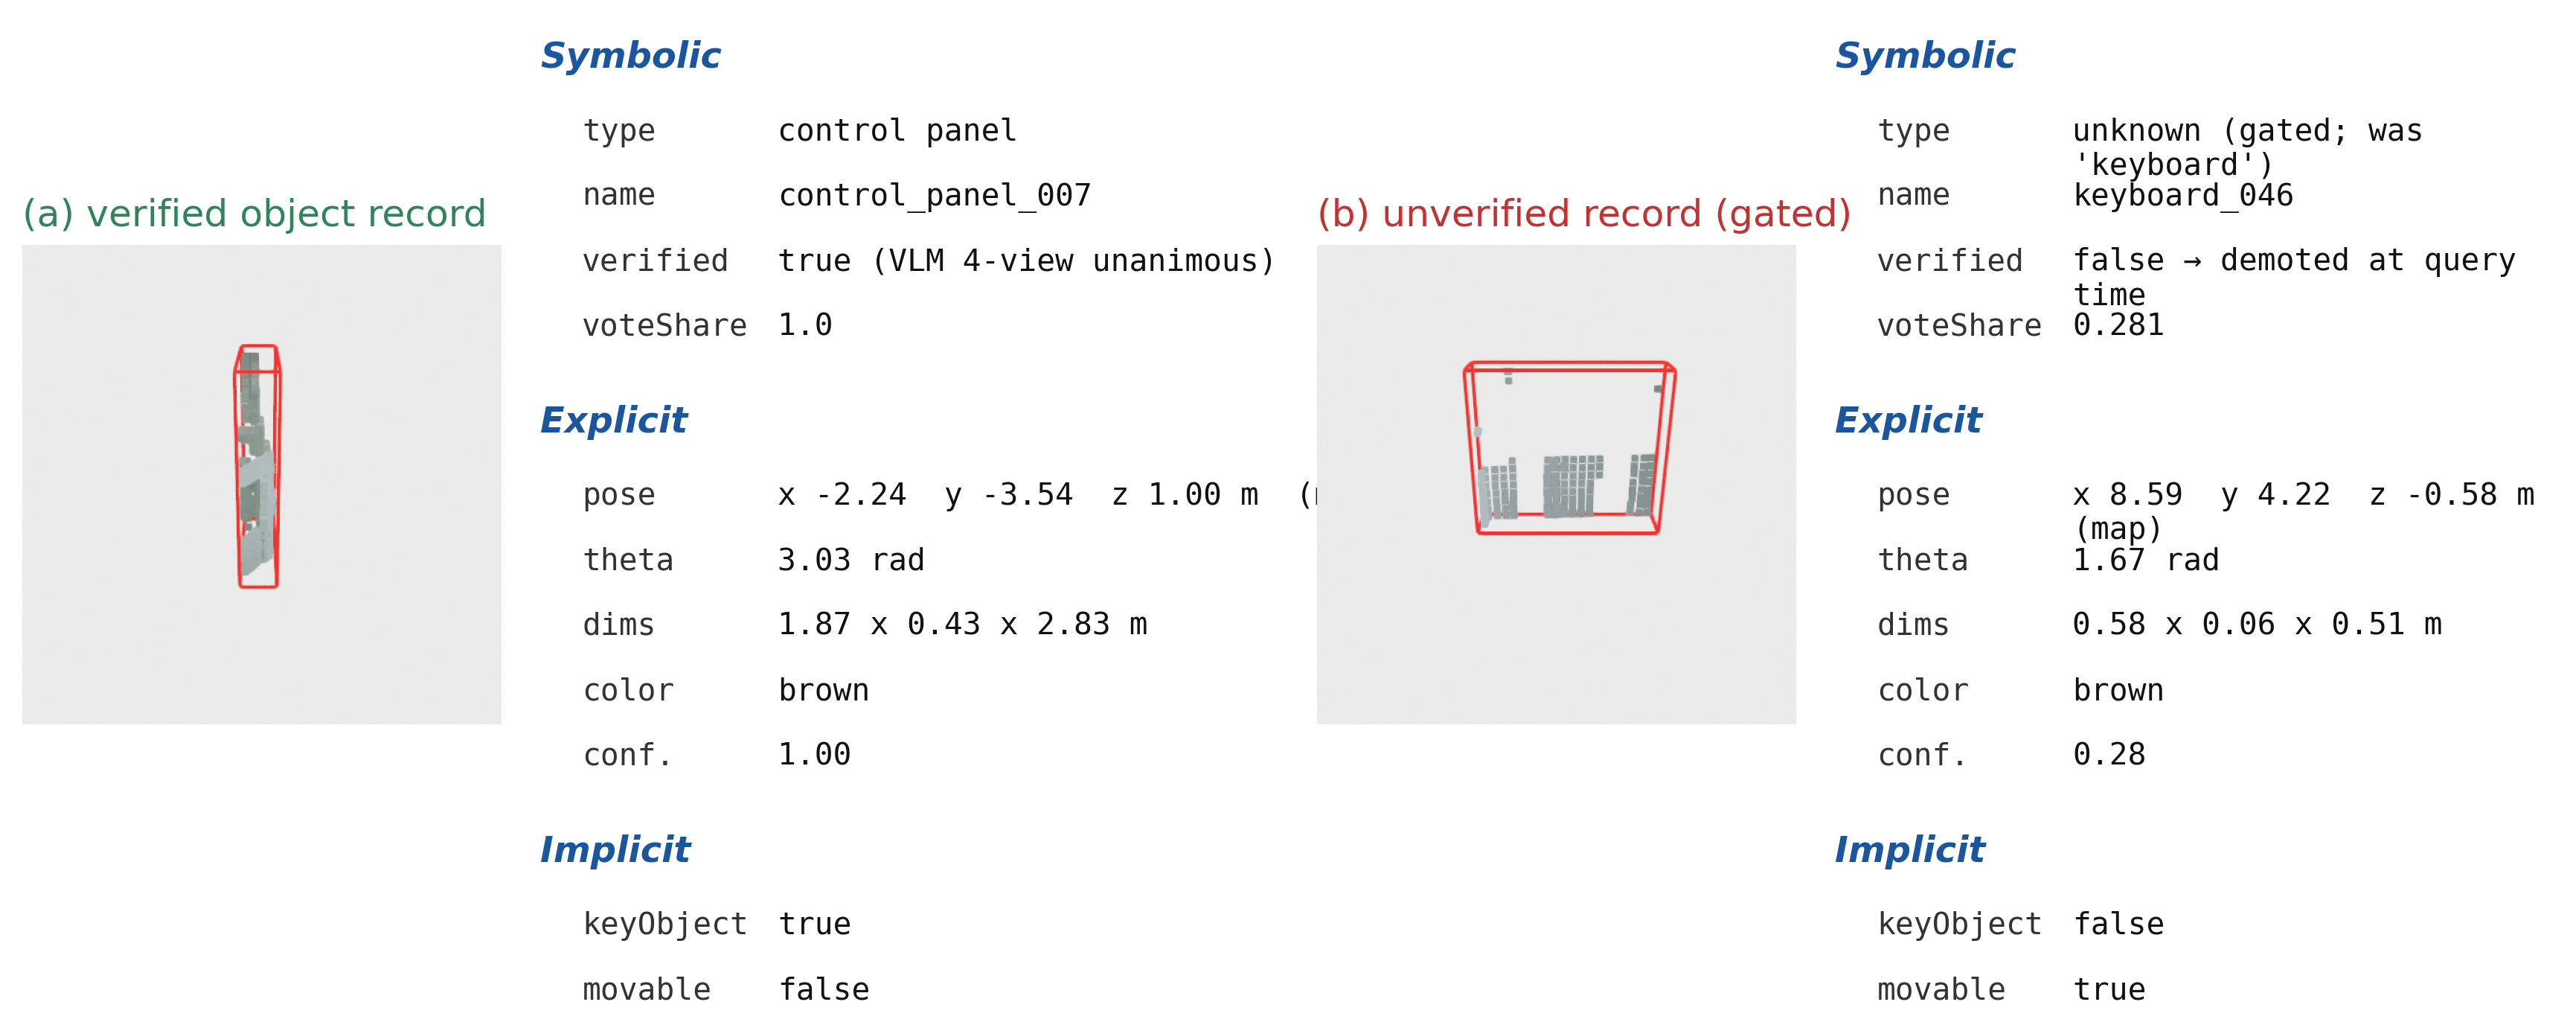
\includegraphics[width=0.95\linewidth]{figures/ele_fig4_record_cards.png}
\caption{TOSM semantic-object records (symbolic / explicit / implicit layers).
(a)~A verified record asserts its type. (b)~An unverified record is
structurally gated at query time: the type is demoted to \texttt{unknown} and
the failed classifier guess is quarantined in \texttt{failedCandidateType}.}
\label{fig:cards}
\end{figure}

\section{Object-Grounded Place Layer}
\label{sec:place}

Robot tasking refers to places (``the docking area'') as often as to objects.
Following the TOSM place schema of DK-SMF~\cite{joo2025dksmf}---boundary
polygon, containment, and purpose---the framework adds a place layer grounded
in the verified object layer. Place regions are obtained automatically from
the robot-facing occupancy grid map (0.05~m; the exploration SLAM map of
Chapter~\ref{ch:mapping} on deployment, or a grid synthesized from the scan's
floor points where no exploration run exists): the room interior delimited by
the mapped outer boundary is partitioned by SLIC superpixel
segmentation~\cite{achanta2012slic} with the number of superpixels as the
governing parameter (seven requested here), fragments below an area threshold
(1.5~m$^2$) are discarded, and each region's centroid is the moment-based
center of its cells (cf.\ grid-map room
segmentation~\cite{bormann2016room,luperto2022robust}). Each object's
\texttt{isInsideOf} resolves to the region containing its anchor cell. Each
place is then summarized by its \emph{ring code}: the sequence of member
objects sorted by bearing around the place centroid---restricted to
verified-tier objects, so the confidence gate propagates into place
semantics---and a single LLM call names the place from its ring code. Because
the segmentation depends only on the map, region identity is stable across
scan epochs, and the same regions re-derive names that track the room's actual
use without manual re-annotation (Section~\ref{sec:exp-update}).
Figure~\ref{fig:placemap} shows the resulting place layer. The robot layer of
TOSM is instantiated from the platform description in
Chapter~\ref{ch:validation}.

\begin{figure}[!htb]
\centering
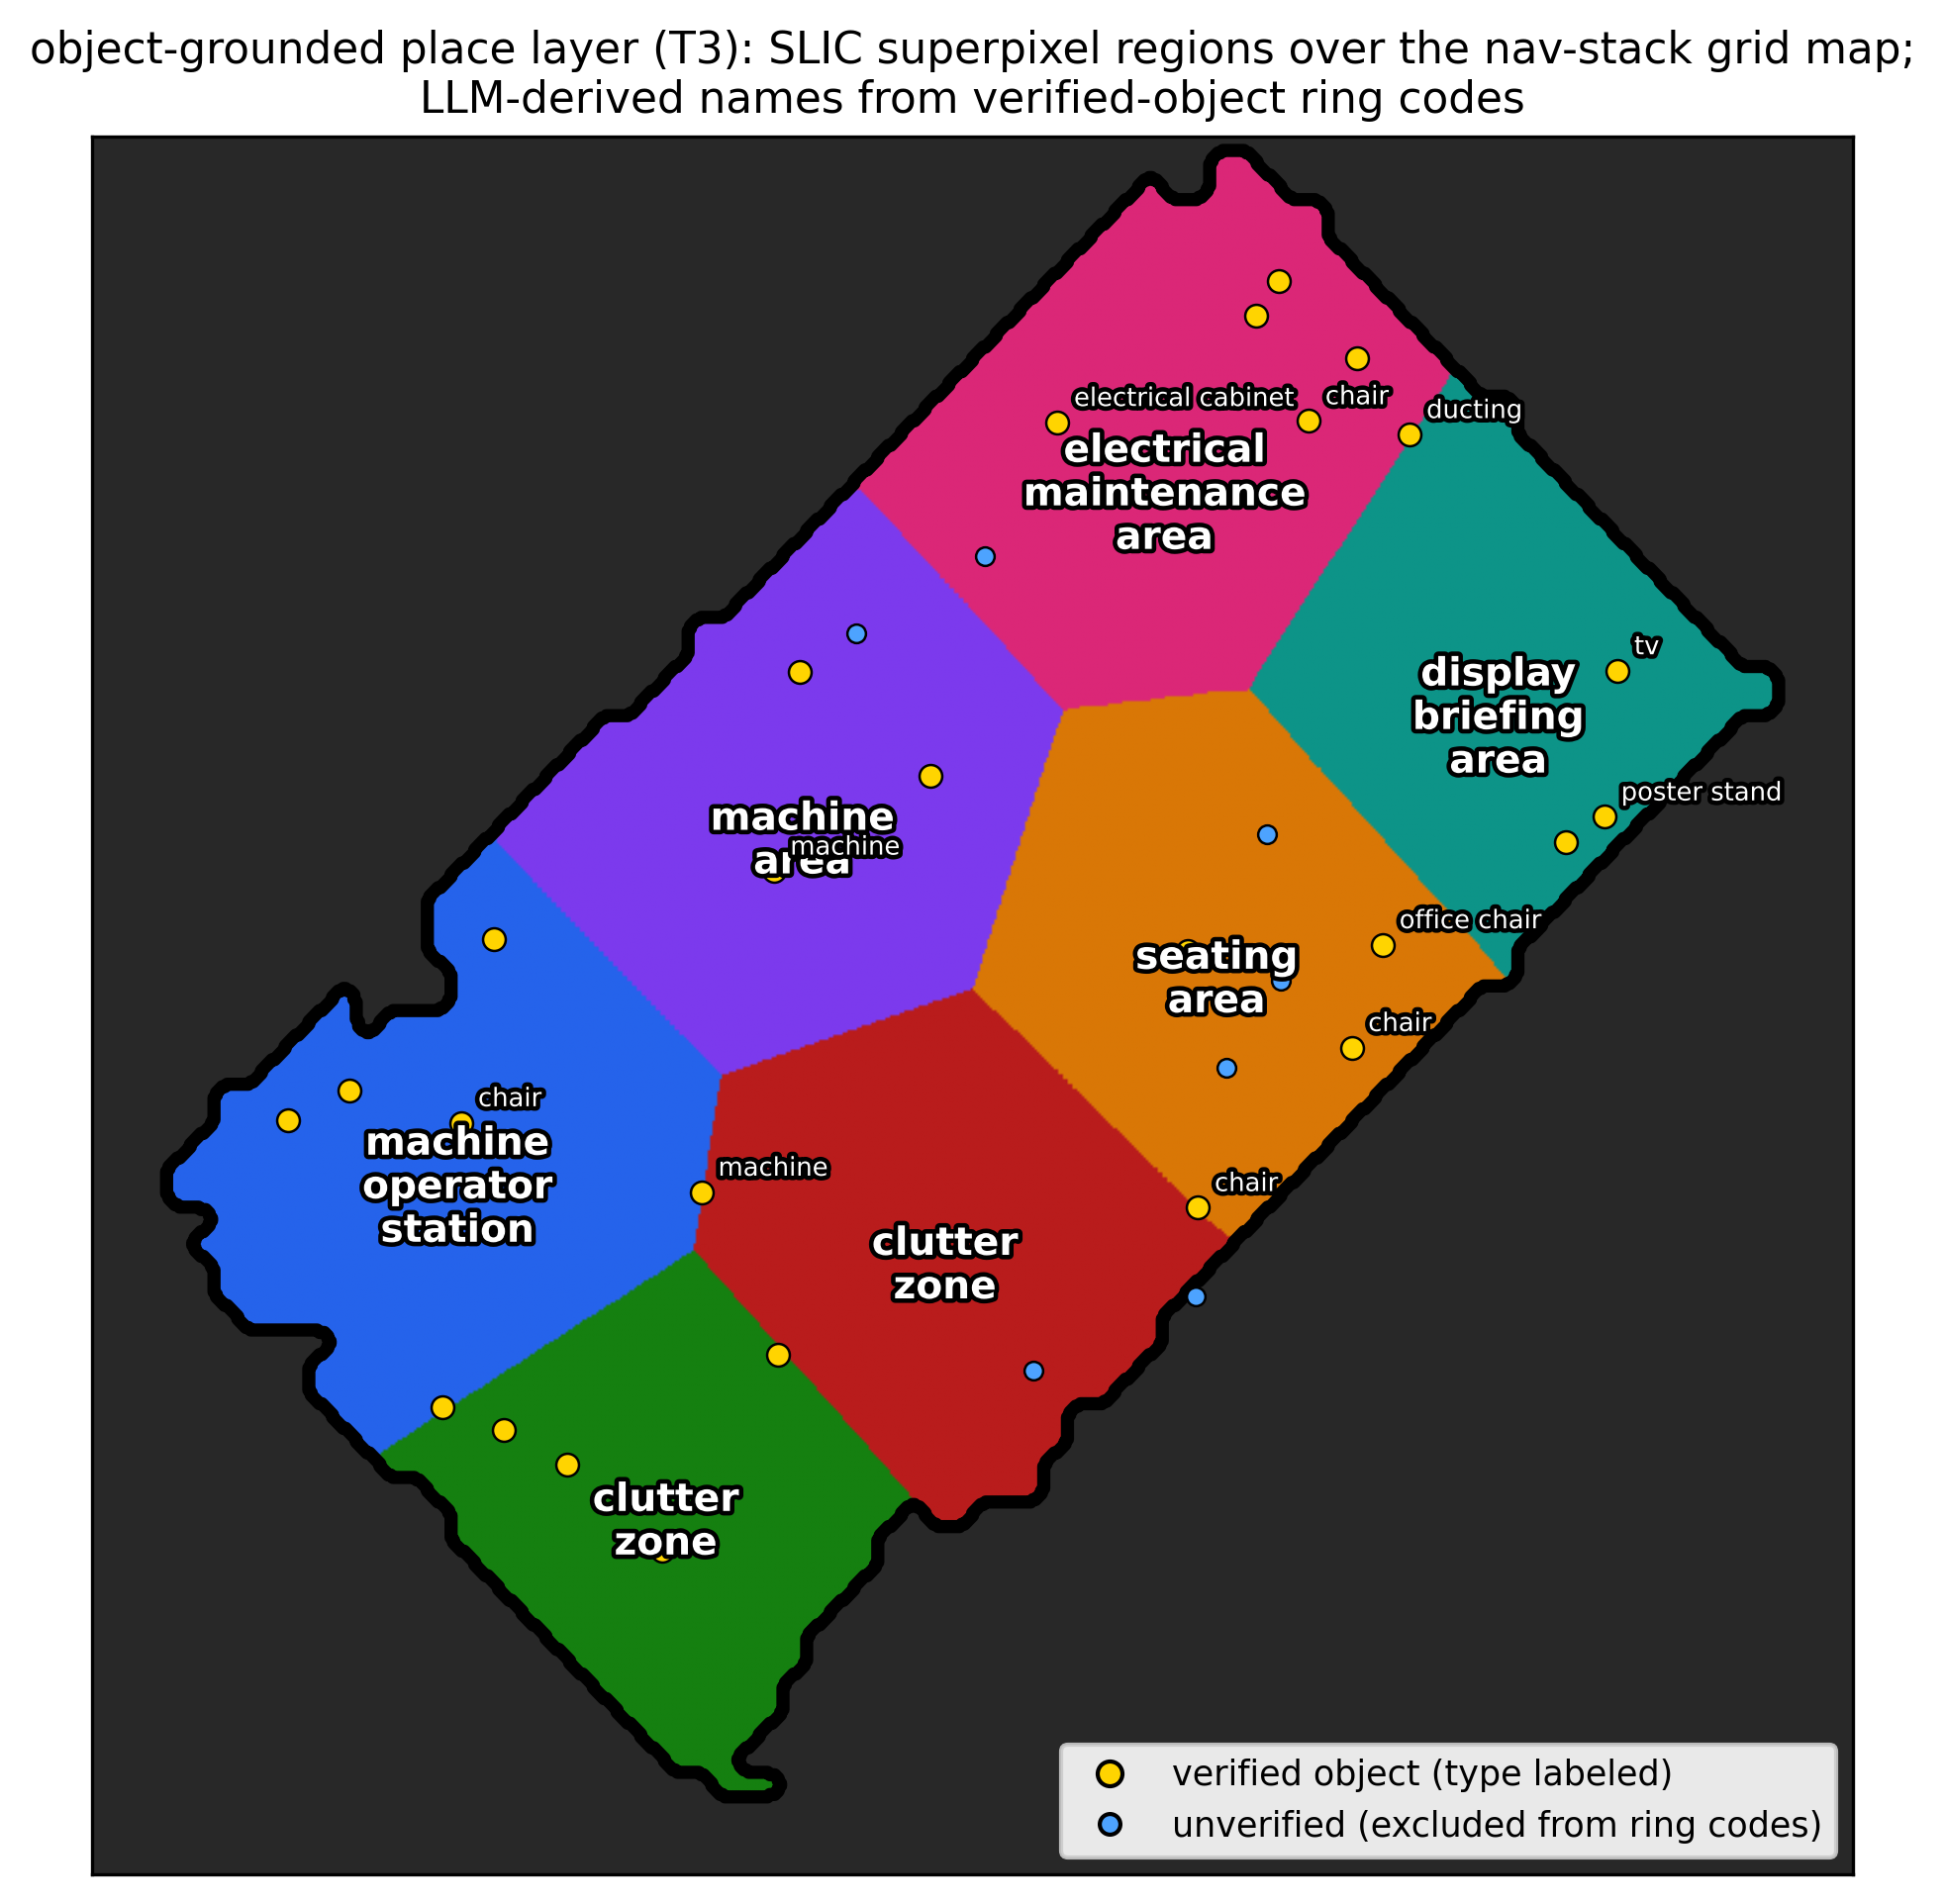
\includegraphics[width=0.85\linewidth]{figures/ele_fig11_place_map.png}
\caption{Object-grounded place layer. SLIC superpixel regions tile the room
interior delimited by the navigation grid map's outer boundary and carry
LLM-derived names computed from verified-object ring codes; unverified objects
(blue markers) do not contribute, so the confidence gate propagates into place
semantics.}
\label{fig:placemap}
\end{figure}

\section{Multilayer Robot-Consumable Representation}
\label{sec:layers}

From the same 3D semantic model, the framework derives the layers that
spatial operations at different heights require, so that the representation
remains compatible with conventional 2D-laser-based navigation stacks while
exposing the vertical structure that a mobile manipulator or a lifting
platform needs (Figure~\ref{fig:layers}). Three vertical bands are defined
relative to the estimated floor plane $z_0$.

\begin{itemize}[leftmargin=2.2em,itemsep=2pt]
  \item \textbf{Driving layer} ($z_0+0.10$ to $z_0+1.80$~m). Points in the
        band relevant to a mobile base are rasterized into a 2D occupancy grid
        at 0.05~m resolution and exported in the ROS map format, so that the
        simulated and real navigation stacks share one map
        (Section~\ref{sec:scan2sim}); the exploration SLAM map of
        Chapter~\ref{ch:mapping} is the equivalent product on a deployment
        where the robot itself mapped the space. The place layer of
        Section~\ref{sec:place} is defined on this grid.
  \item \textbf{Manipulation work layer} (reach band of the platform,
        $z_0+0.4$ to $z_0+1.6$~m for the AMMR). The explicit models of every
        verified object whose extent intersects the band provide the
        footprints, poses, top heights, and movability from which a mission
        mediator computes approach poses and clearance checks against the
        robot's own footprint (Section~\ref{sec:missions}) and from which a
        manipulation planner screens coarse feasibility; no separate
        rasterization is needed because the object records already carry
        metric 3D extents.
  \item \textbf{Overhead layer} (above the driving band, up to the ceiling).
        Ceiling-mounted structure---fixtures, ducts, cable trays, beams, and
        installation targets---is recognized by the overhead recognition
        module of Section~\ref{sec:overhead} from the pre-removal ceiling
        reference cloud that the backbone retains, verified under the same
        protocol, and merged into the graph with \texttt{heightLevel = high},
        so that a pointing or installation task can be resolved to a metric
        overhead target in the map frame.
\end{itemize}

Each band is a view over one graph rather than a separate model: an object
record carries its full 3D extent, and band membership is a query. The
simulation layer of Chapter~\ref{ch:validation} injects the same records
into a physics-enabled stage. The driving band and the place layer are
exercised end to end on the physical robot in Section~\ref{sec:exp-missions};
the overhead band is evaluated in Section~\ref{sec:exp-overhead}.

\begin{figure}[!htb]
  \centering
  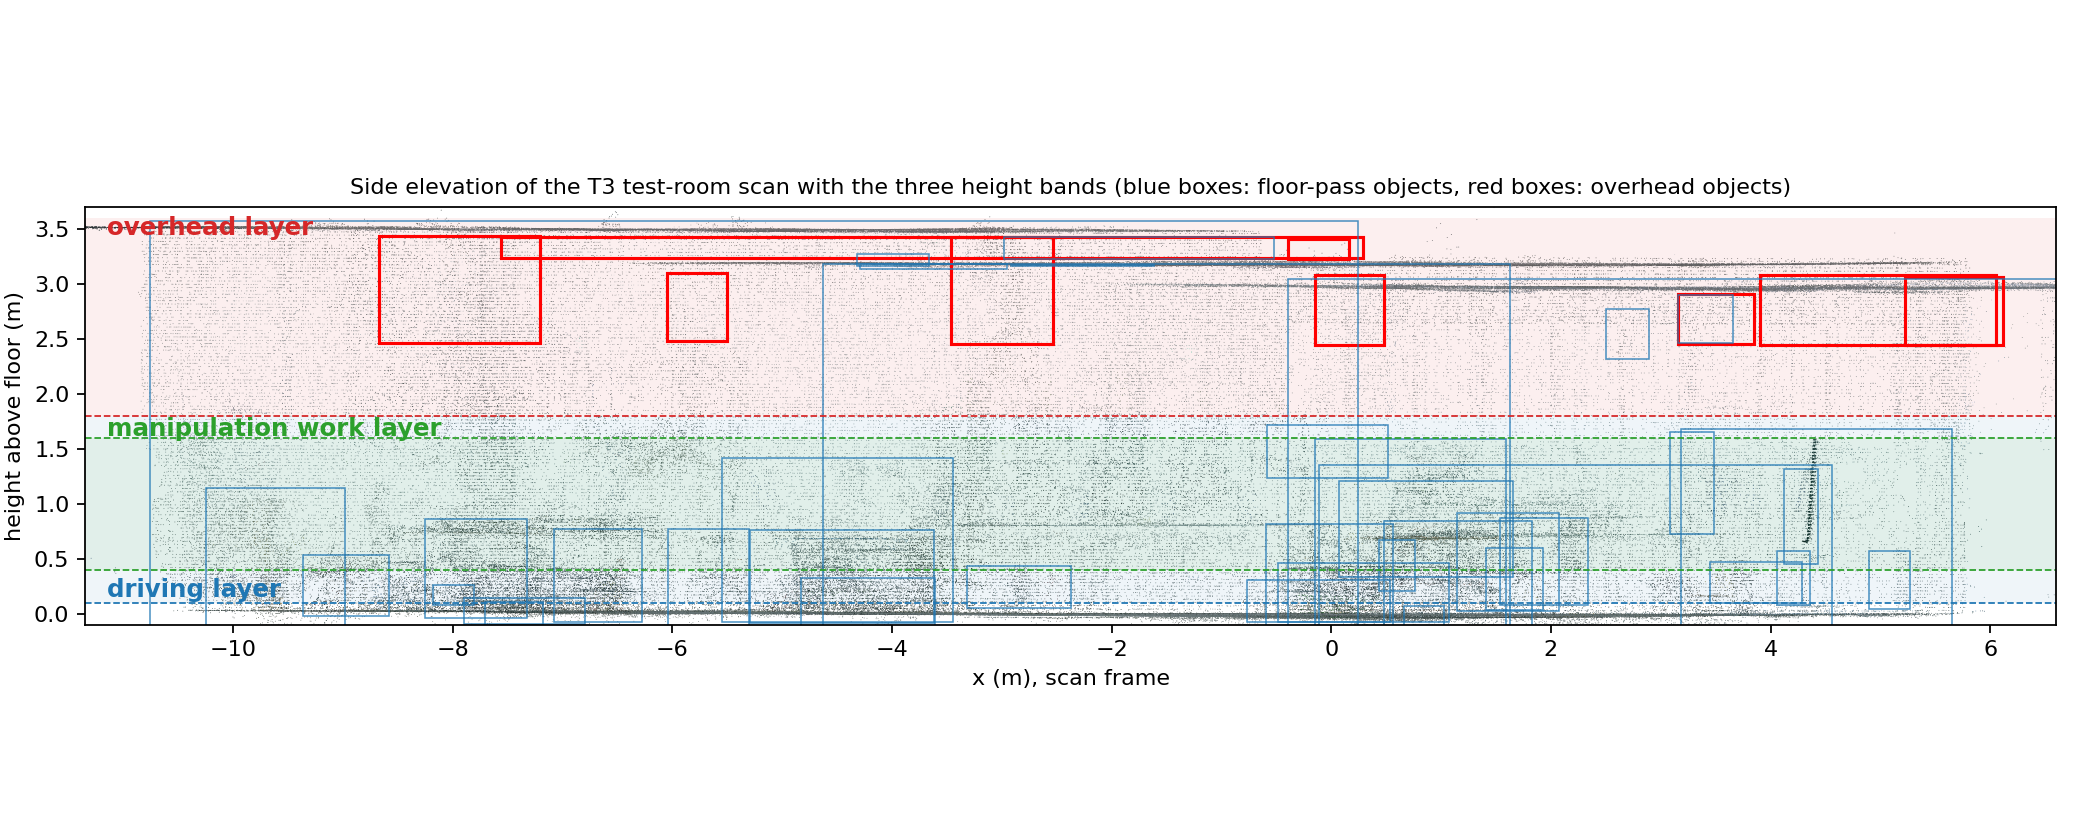
\includegraphics[width=0.95\textwidth]{figures/fig4_layers.png}
  \caption{Multilayer robot-consumable representation. The driving layer
  (occupancy grid and place layer), the manipulation work layer (verified
  object extents at reach height), and the overhead layer (ceiling-mounted
  structure from the overhead recognition module) are three height-band views
  over the one knowledge graph; a mobile manipulator consumes all three.}
  \label{fig:layers}
\end{figure}

\section{Overhead Structure Recognition}
\label{sec:overhead}

A strength of survey-grade TLS is that it captures the ceiling as faithfully
as the floor, yet the backbone of Section~\ref{sec:backbone} removes the
ceiling planes and discards everything attached to them in order to isolate
floor-standing objects. The overhead recognition module recovers that
content as a complementary pass that is appended to the frozen pipeline and
merged with the floor-level graph, without altering the object-level
algorithm validated in Sections~\ref{sec:exp-seg}--\ref{sec:exp-endtoend}.

The module operates on the pre-removal \emph{ceiling reference} cloud that
the backbone retains (Section~\ref{subsec:preprocess}), colored from the raw
scan by the same deterministic downsampling, and proceeds in six steps with
the parameters fixed once and applied unchanged to every scene.
\begin{enumerate}[leftmargin=2.2em,itemsep=2pt]
  \item \emph{Overhead band.} The floor height is estimated as in the
        remnant filter, and only points more than 1.80~m above it---the top
        of the driving band---enter the pass.
  \item \emph{Ceiling levels.} Near-horizontal planes ($|n_z|\ge0.85$) are
        extracted from the band by the same seeded RANSAC as the structure
        removal, up to four levels, so that multi-level ceilings are
        represented explicitly; points within $\pm0.06$~m of a level are
        ceiling and are excluded, as is content above the highest level
        (seen through openings).
  \item \emph{Walls.} Near-vertical planes ($|n_z|\le0.2$) are extracted from
        the remaining band points, up to eight; points within 0.12~m of a
        wall plane are wall.
  \item \emph{Floor-object exclusion.} Points that fall inside the padded
        (0.10~m) footprint of a floor-pass object and below that object's top
        are the upper part of an object the floor pass already owns and are
        excluded; merged clusters wider than 3~m are ignored for this test so
        that a mega-cluster's footprint cannot swallow the ceiling.
  \item \emph{Decomposition and explicit model.} The remaining candidates
        are clustered by the floor pass's DBSCAN ($\varepsilon=0.30$~m, 80
        points minimum) with the same conservative giant-split, and each
        cluster receives the same explicit model (extent, centroid, yaw,
        color) plus three overhead attributes: the clearance below it (bottom
        above floor), the gap to the nearest ceiling level, and its
        attachment---\emph{ceiling-hung} if its top is within 0.15~m of a
        ceiling level, \emph{wall-mounted} if at least 25\% of its points lie
        within 0.22~m of a wall plane, and \emph{suspended} otherwise. The
        height level is \texttt{high} by construction. Candidates are
        room-scoped with the same mask as the floor pass, with a 0.5~m
        tolerance because wall-hung fixtures sit at the free-space boundary.
  \item \emph{Verification and merge.} A provisional label is attached by
        the same open-vocabulary classifier over an overhead vocabulary
        (light fixture, fluorescent lamp, air conditioner, ventilation duct,
        cable tray, beam, pipe, sprinkler head, projector, speaker, sign,
        surveillance camera, smoke detector, ceiling panel, curtain rail),
        the four base views and the eight escalation views are rendered from
        $30^\circ$ \emph{below} the object instead of $25^\circ$ above, and
        the late-fusion verifier of Section~\ref{sec:verification} runs
        unchanged except that the overhead vocabulary is passed as the
        candidate list and the \texttt{high} height level as a hard prior.
        Verified overhead objects enter the graph through the identity
        policy and confidence-gated upsert of
        Sections~\ref{sec:matching}--\ref{sec:upsert}, so that they are
        tracked across epochs like any other node; their spatial relations
        are limited to \texttt{isAboveOf} the floor-level object or place
        beneath them, which is what an installation or pointing task
        consumes.
\end{enumerate}
The structure-remnant and hybrid grid-map filters remain in force for the
floor pass and are not applied to the overhead pass, whose whole purpose is
the content those filters discard; conversely, nothing the overhead pass
finds can alter a floor-pass node, so the evaluation of
Sections~\ref{sec:exp-seg}--\ref{sec:exp-endtoend} is unaffected by enabling
it. Section~\ref{sec:exp-overhead} evaluates the pass on the two industrial
epochs and the cafeteria scene.
